\chapter{Background Estimation}
\label{chap:bkg}

Due to the lifetime ($c\tau > 2$ mm) and mass ($m > 10$ GeV) requirements applied at vertex selection, no SM background is expected in the signal region in search for displaced dilepton resonance. Therefore, two non-collision backgrounds are considered in this search: cosmic background and \textit{random-crossing} background. The cosmic background is the dominant background in this analysis and is estimated. In Section~\ref{sec:bkg:cosmic}. In Section~\ref{sec:bkg:random}, background from random-crossing of two uncorrelated tracks are estimated.


\section{Cosmic Background}
\label{sec:bkg:cosmic}

A cosmic muon passing through the ID during a collision event can be reconstructed as a back-to-back muon pair with opposite electric charges, forming a displaced \mumu vertex.

This cosmic background is suppressed by implementing the cosmic veto, $R_{\mathrm{CR}} < 0.01$ (Section~\ref{sec:event_selection}). The event cut flow in Figure~\ref{subfig:event_cutflow_MC} shows that the cosmic veto is very effective with negligible signal loss. To illustrate the effectiveness of the veto, a cosmic control region is defined as follows:

\begin{itemize}
  \item Events are required to fail the cosmic veto.
  \item Events are required to have at least two muons satisfying vertex track selection (Table~\ref{table:vertex_track_selection_simple}).
  \item All other event selections are kept the same as the signal region.
\end{itemize}

In this control region, pairs of two muons with leading $p_{T}$ are studied using the data sample. Figure~\ref{fig:cosmicData} shows the distribution of the pairs in $|\Delta\phi|$ and $\Sigma \eta$. The distribution shows that a significant faction of muons pairs is from cosmic rays and is constraint to the small \Rcr region.

\begin{figure}[!htb]
    \begin{center}
    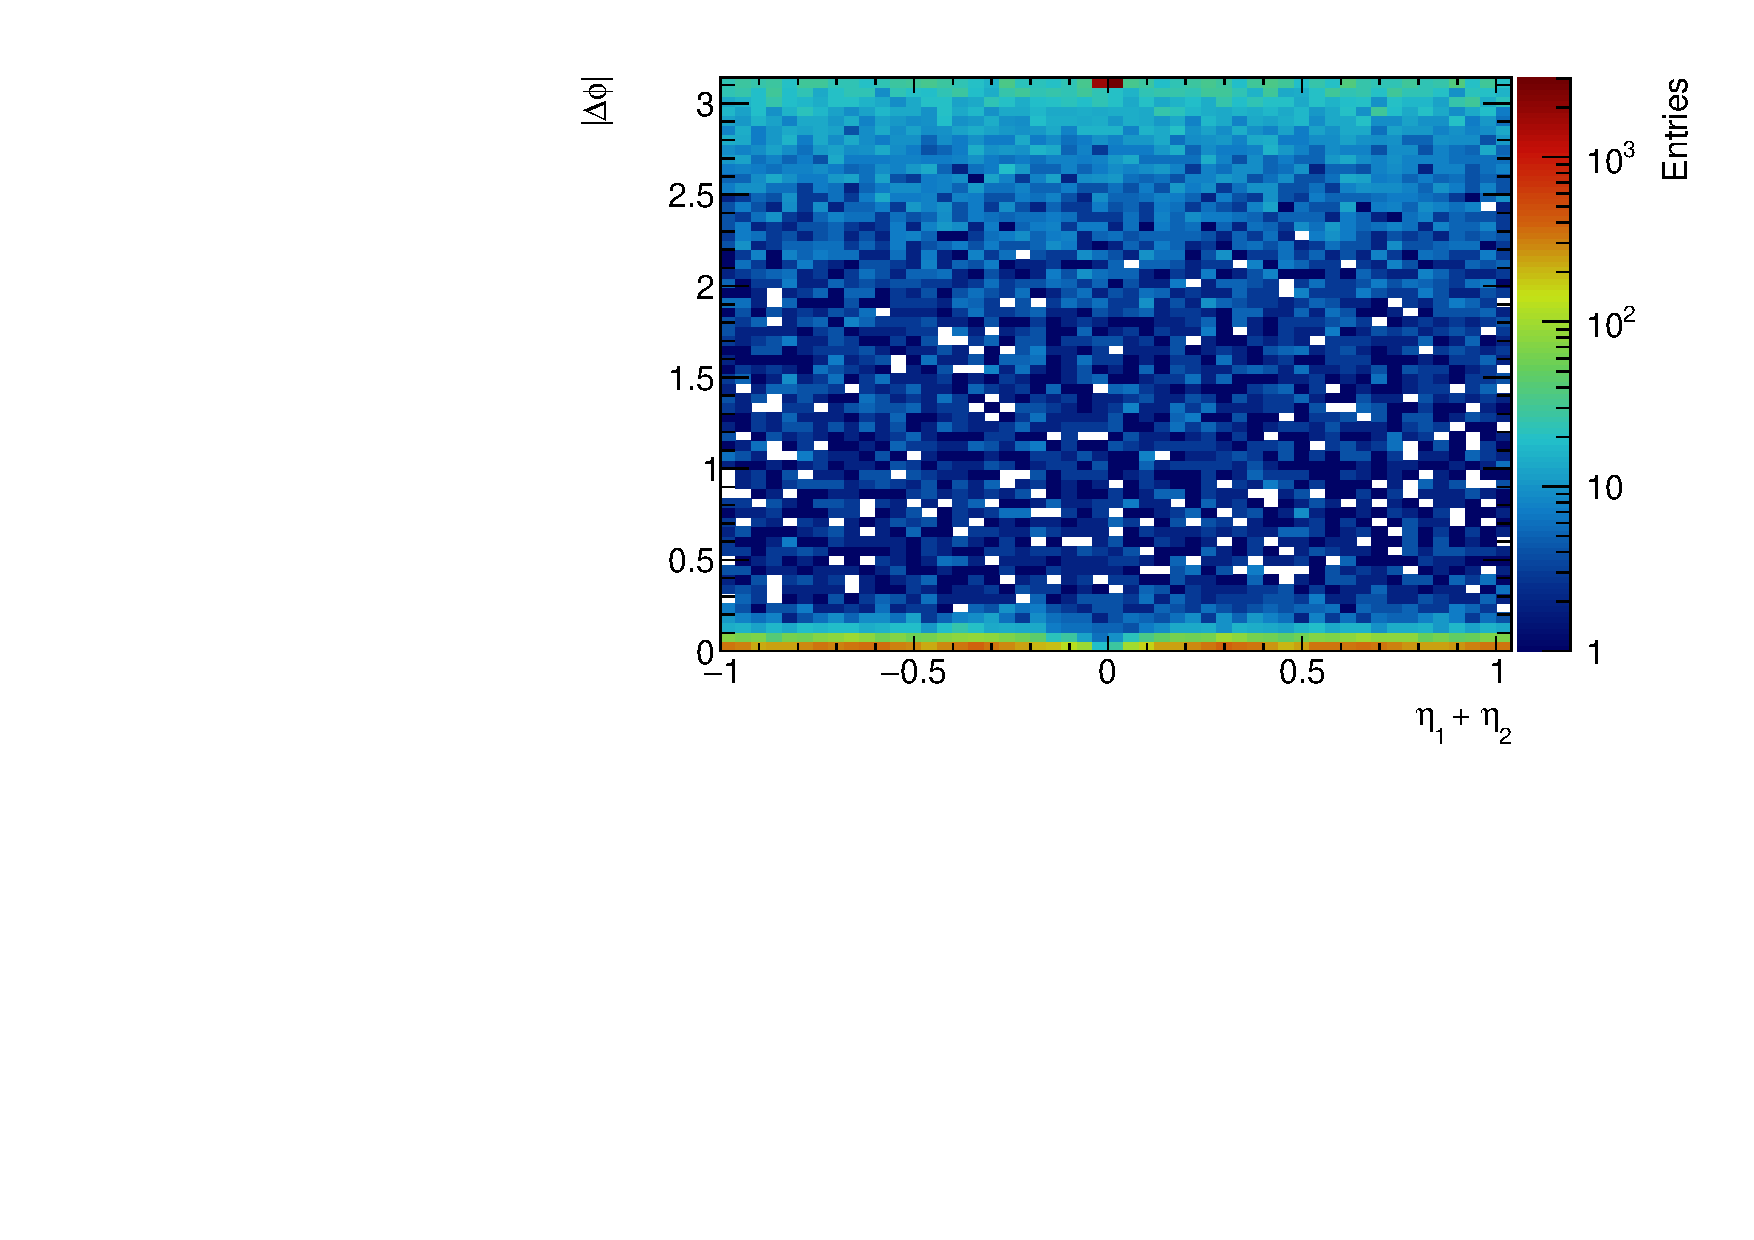
\includegraphics[width=0.6\textwidth]{figures/Cosmics/DataValidation/mup_seta_dphi.pdf}
    \label{fig:cosmicData}
    \caption{Distribution of pairs of two muons with leading $p_{T}$ in $|\Delta \phi|$ and $\Sigma \eta$ found in the cosmic control region using the data sample. The sharp peak at $|\Delta\phi| = \pi$ and $\Sigma \eta = 0$ shows that a significant fraction of muon pairs in the region is from cosmic muons.}
\end{center}
\end{figure}

To estimate the cosmic background in the signal region, the \Rcr distribution of \mumu pairs is compared to those forming a vertex in Figure~\ref{fig:cosmicCRb}. There are 246 \mumu vertices found in the data sample that pass all of the signal selection except the cosmic veto, and there is no event with \Rcr > 0.004, indicating that the cosmic background is effectively suppressed by the cosmic veto of \Rcr = 0.01.

The \Rcr distribution, normalized to \mumu pairs forming a vertex, yields a cosmic background of 0.27$\pm$0.14 (stat.). This background is about two orders of magnitude larger than the random crossing background. Therefore, the cosmic muon background is the dominant source of background in the signal region.


\begin{figure}[!htb]
    \centering
    \subfloat[Unscaled\label{fig:cosmicCRa}]{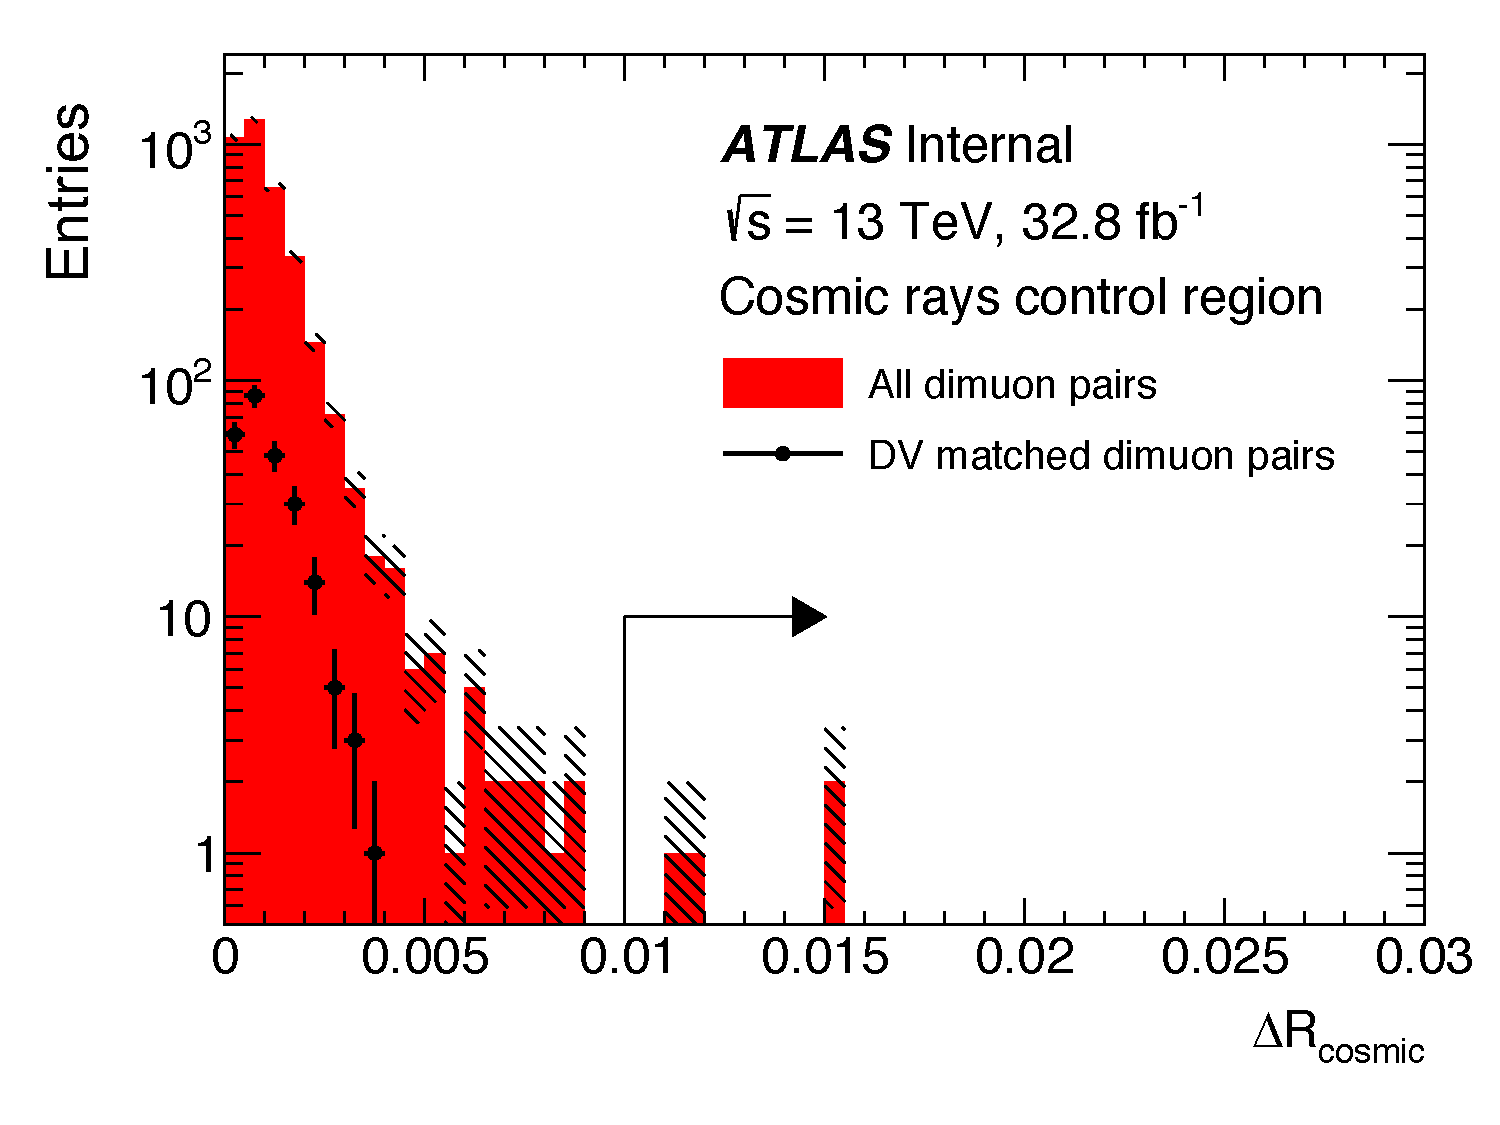
\includegraphics[width = 0.49 \textwidth]{figures/Cosmics/DataValidation/cosmics_unscaled.pdf}}
    \subfloat[Scaled\label{fig:cosmicCRb}]{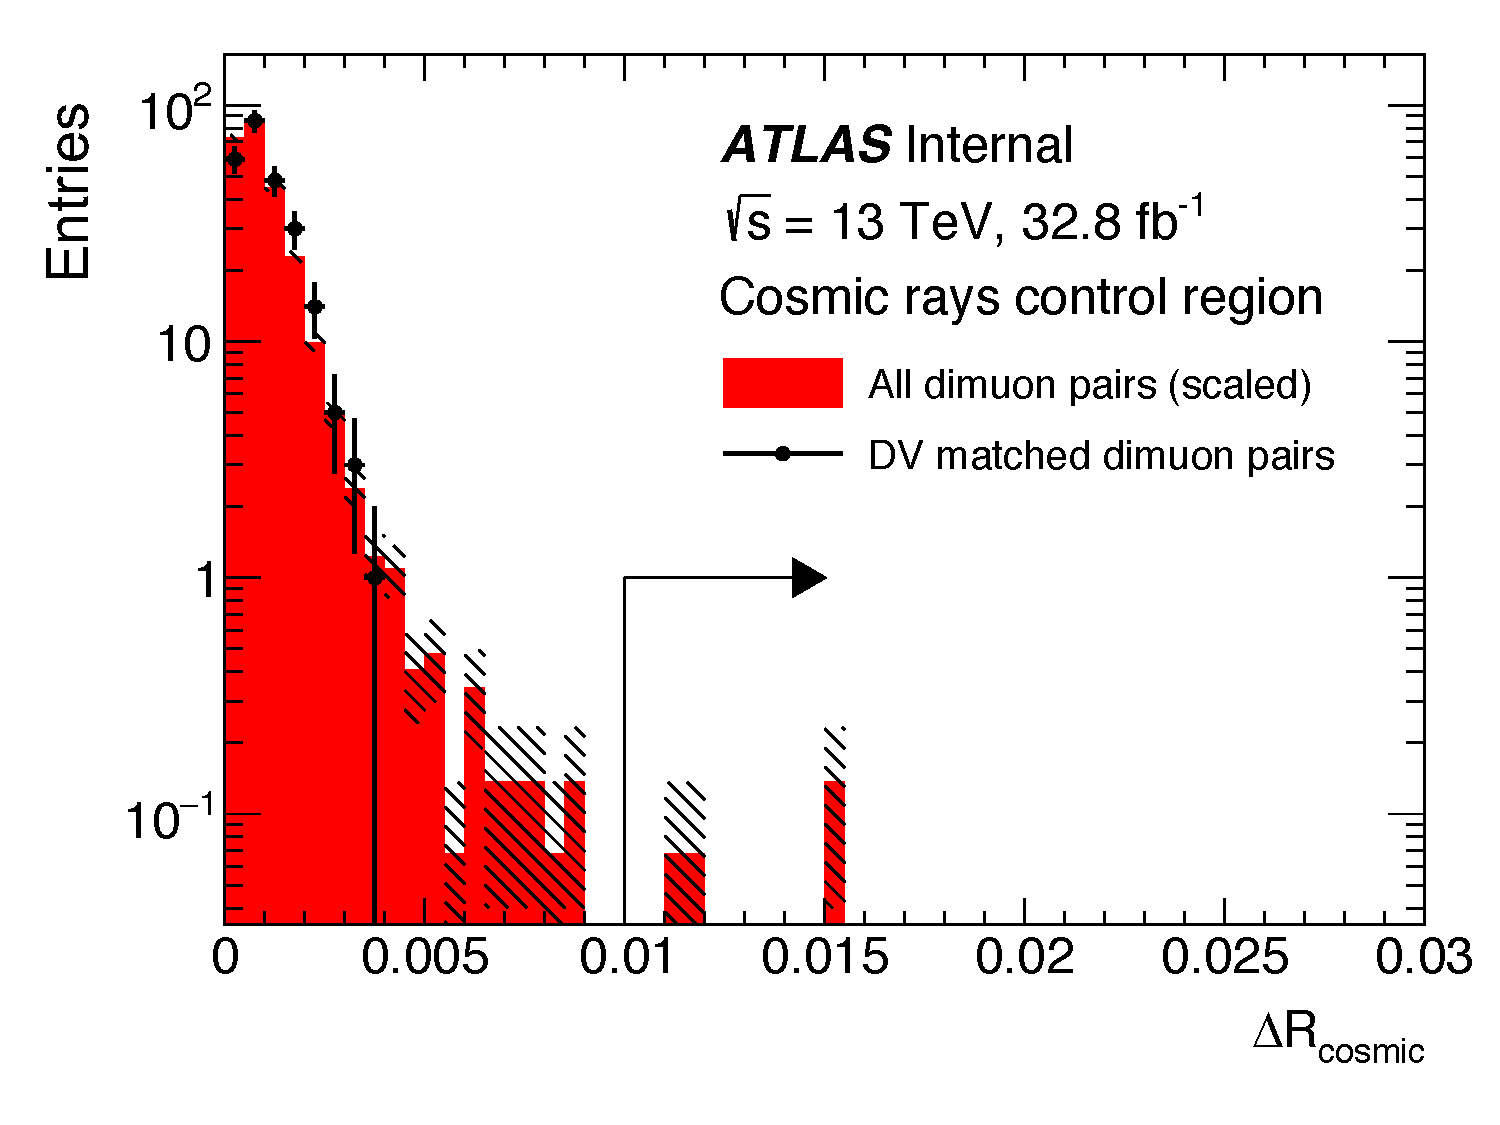
\includegraphics[width = 0.49 \textwidth]{figures/Cosmics/DataValidation/cosmics_scaled.pdf}}
    \label{fig:cosmicCR} 
	\caption{Comparison of the \Rcr distribution of \mumu pairs with (dots) and without (shaded) the vertex requirement. The same distribution is shown in (b) normalized to the number of \mumu pairs forming a vertex.}
	%\caption{(a) Distribution of \mumu vertices and pairs from the data sample in small \Rcr region. The red distribution represents all \mumu pairs. The black dots represent the subset of pairs forming a \mumu vertex. The same distribution is shown in (b) with \mumu pairs normalized to \mumu vertices.}
\end{figure}



\section{Random-Crossing Background}
\label{sec:bkg:random}

The random-crossing of two uncorrelated tracks can be a major source of the backgrounds in the search for displaced dilepton vertices. This background is expected to increase with more pile up in Run 2.
 
This random-crossing background is estimated by a data-driven method called the \textit{track flipping} (TF). In this method, secondary vertex reconstruction is performed on each pair of tracks from all possible combinations of tracks after one random track from each pair is flipped with respect to the beam spot. Because one track is flipped in each pair of tracks, the resulting vertices provide good estimation for random-crossing background. In addition, another random-crossing background method called the \textit{Event mixing} is used to estimate systematic uncertainty in the background estimation.

The TF and event mixing methods are described in Section~\ref{sec:bkg:random_crossing_tf} and ~\ref{sec:bkg:random_crossing_em}, respectively. In Section~\ref{sec:bkg:random_crossing_MC}, the TF method is tested on the background MC samples, and the result is compared with the corresponding result from the event mixing. In Section~\ref{sec:bkg:random_crossing_data}, the random-crossing background in data is estimated by the TF method.%, and its systematic uncertainty is estimated by comparing the estimation from the TF and event mixing in Section~\ref{sec:bkg:random_crossing_syst}.

\subsection{Track Flipping Method}
\label{sec:bkg:random_crossing_tf}

In the TF method, events are selected by the same requirement described in Section~\ref{sec:selection:pre}. From the selected events, ID tracks associated with a muon, electron, or neither, referred as muon, electron, or non-leptonic track, respectively, are selected with the track criteria (Table~\ref{table:vertex_track_selection_simple}) used for the secondary vertexing algorithm. Lepton tracks are required to pass the same selection criteria described in Table~\ref{table:lepton_requirement}. Non-leptonic tracks are required to pass the same kinematic selection ($p_{T} > 10$ GeV, $|\eta| < $ 2.5) as leptons.

\begin{figure}[!htb]
    \subfloat[]{\label{subfig:TF_diagram_a}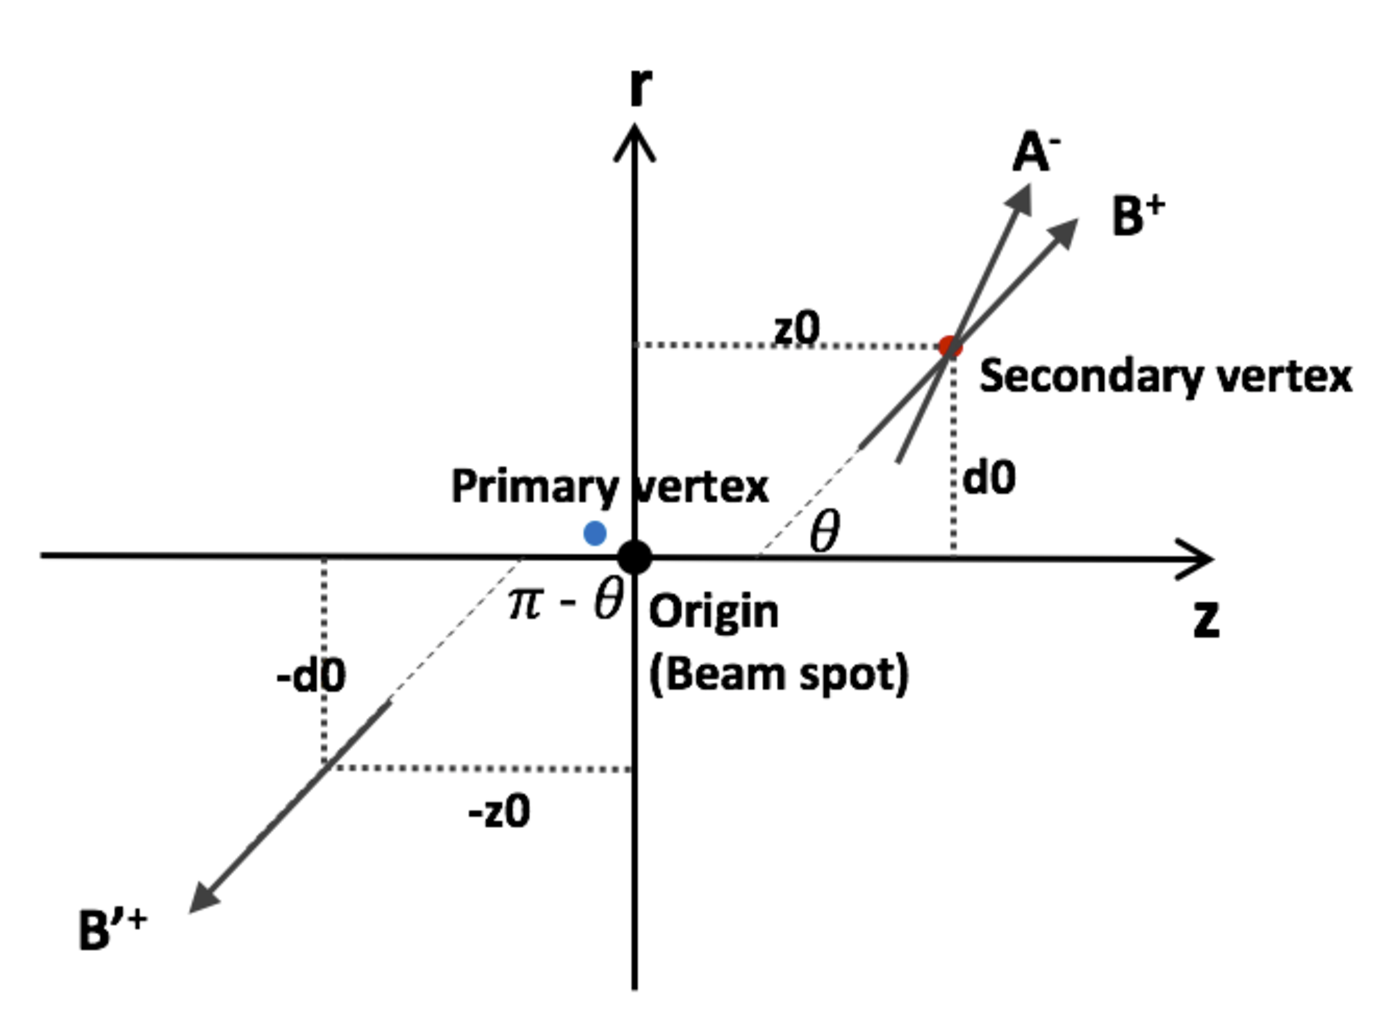
\includegraphics[width=0.50\textwidth]{figures/TF_diagram_a.pdf}}
    \subfloat[]{\label{subfig:TF_diagram_a}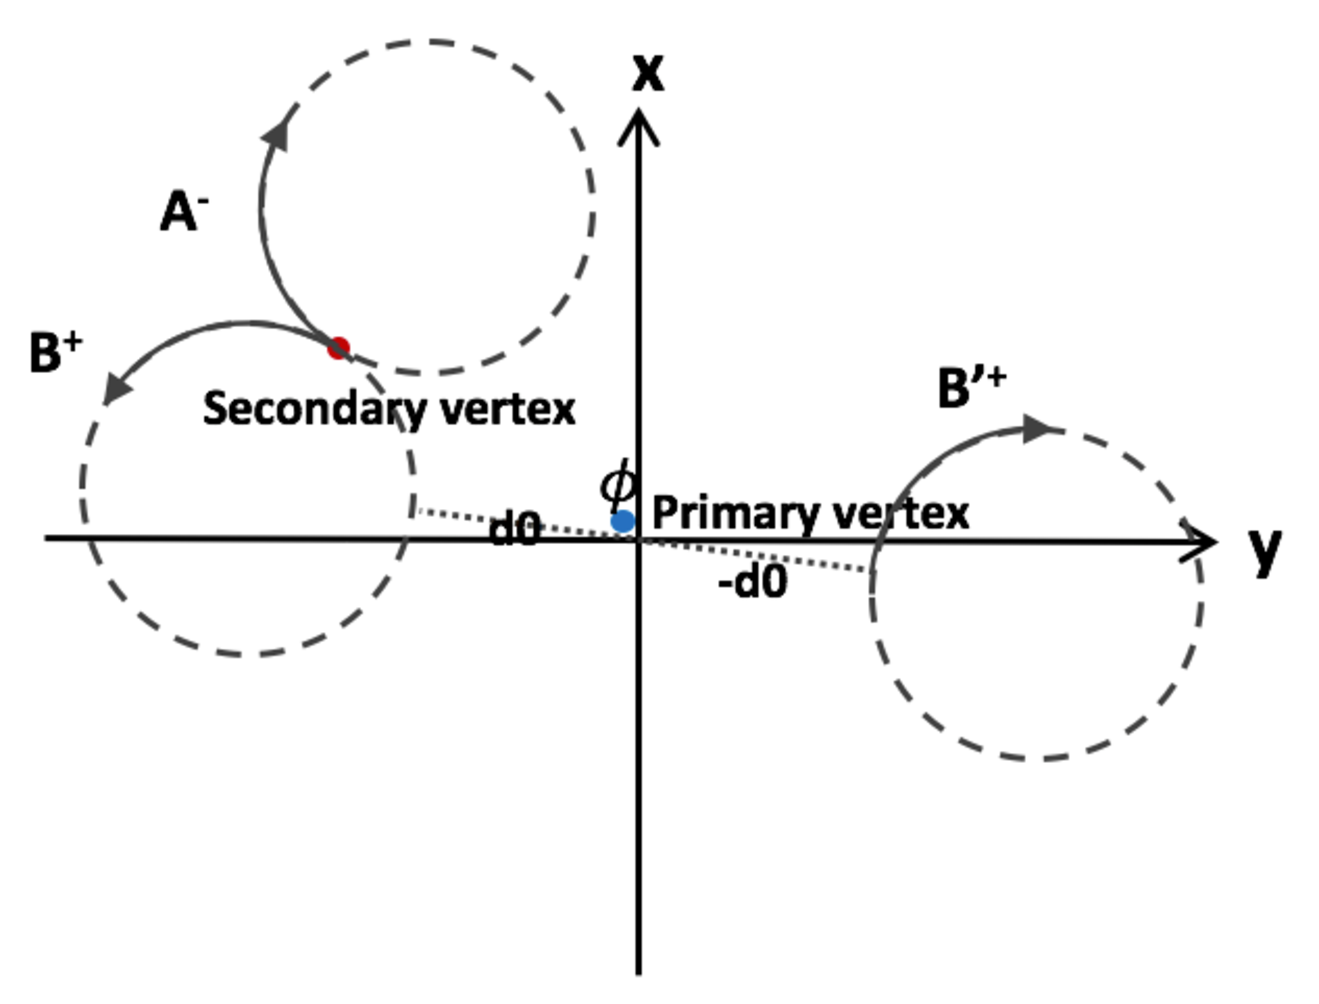
\includegraphics[width=0.50\textwidth]{figures/TF_diagram_b.pdf}}
	\centering
	\caption{Description of track flipping method in (a) $r-z$ and (b) $x-y$ plane. Given two tracks $A$ and $B$ originating from a common secondary vertex, one random track is flipped with respect to the beam spot and is denoted as $B'$. The resulting flipped track pair, $AB'$, cannot form a vertex due to the separation in space.}
	\label{fig:TF_diagram}
\end{figure}

From the selected tracks, track pairs are created from all possible combination of muon, electron, or non-leptonic tracks, i.e. \mumu, \ee, \emu, \ex, \mux, or \xx, where x represents a non-leptonic track. For each pair of tracks, one random track is flipped with respect to the beam spot ($\dzero \rightarrow -\dzero, \zzero \rightarrow -\zzero, \phi\rightarrow\phi+\pi, \theta\rightarrow\pi-\theta$), creating a \textit{flipped track pair}. The secondary vertex algorithm used in the reconstruction of data or MC sample is used to reconstruct displaced vertices using these flipped track pairs. Vertex selection cuts similar to the cuts listed in Table~\ref{table:vertex_track_selection_simple} are applied to the vertices found from flipped track pairs, except that the trigger matching and filter matching are only required for $\mu\mu$, $ee$, and $e\mu$. 

Track-flipped vertices are formed purely from random-crossing of tracks as depicted in Figure~\ref{fig:TF_diagram}. Therefore, track-flipped vertex yields provide a good estimation for random-crossing background. Also, because trigger and filter matchings are not imposed in the control and validation region, the TF method provides conservative background estimation. 



\subsection{Event Mixing Method}
\label{sec:bkg:random_crossing_em}

The event mixing method is similar to the TF, but instead of flipping a track from pair of tracks, it combines tracks from different events to create uncorrelated track pairs, i.e. two tracks are not originating from a real vertex.

The event mixing method proceed as follows. First, muon, electron, and non-leptonic tracks that satisfy the track criteria (Table~\ref{table:vertex_track_selection_simple}) are collected from all events, resulting in a collection of all potential seed objects in the sample. Lepton tracks are required to pass the same selection criteria\footnote{Only lepton pairs with an invariant mass greater than $6~\si{\GeV}$ are used in the normalization procedure to remove any contamination from low mass processes.} described in Table~\ref{table:lepton_requirement}. Non-leptonic tracks are required to pass the minimal kinematic selection ($p_{T} > 10$ GeV, $|\eta| <$ 2.5 to match with the kinematic selection for leptons.

Pairs of tracks are randomly sampled from the collection. For each track pair, a primary vertex is randomly chosen from all events with a lepton candidate. Primary vertices are needed in order to evaluate the displacement cut and quality requirements of the vertexing algorithm. The secondary vertex reconstruction is performed on each track pair.

The ratio of event-mixing vertex yields to the number of track pairs sampled represents the probability, $p_{\mathrm{xing}}$, of two tracks randomly forming a displaced vertex. Using $p_{\mathrm{xing}}$ and the total number of track pairs of each type (\mumu, \ee, \emu, \mux, \ex, \xx) in data, the random-crossing background is estimated for each type by, e.g.,

\begin{equation}
    N_{\mumu}^{v} = N_{\mumu} \times p_{\mathrm{xing}},
\label{eq:N_Comb_Vertices}
\end{equation}
%
where $N_{\mumu}^{v}$ represent the estimated random-crossing background of \mumu type, and $N_{\mumu}$ represents the total number of \mumu pairs present in data. The random-crossing probability, $p_{\mathrm{xing}}$, is estimated individually for each type of vertices. The details on this method can be found in Ref.~\cite{DuarteCampderros:2275055}.







\subsection{MC Study}
\label{sec:bkg:random_crossing_MC}
The TF method is tested using the background MC sample described in Section~\ref{sec:background_mc_sample}, and the resulting vertex yields and distributions are compared with the corresponding result from event mixing method. A representative plot of vertex cut flows in the TF method is shown in Figure~\ref{fig:m_FBE_cutflow_MC} using track-flipped \xx vertices from the background MC samples.

\begin{figure}[!htb]
	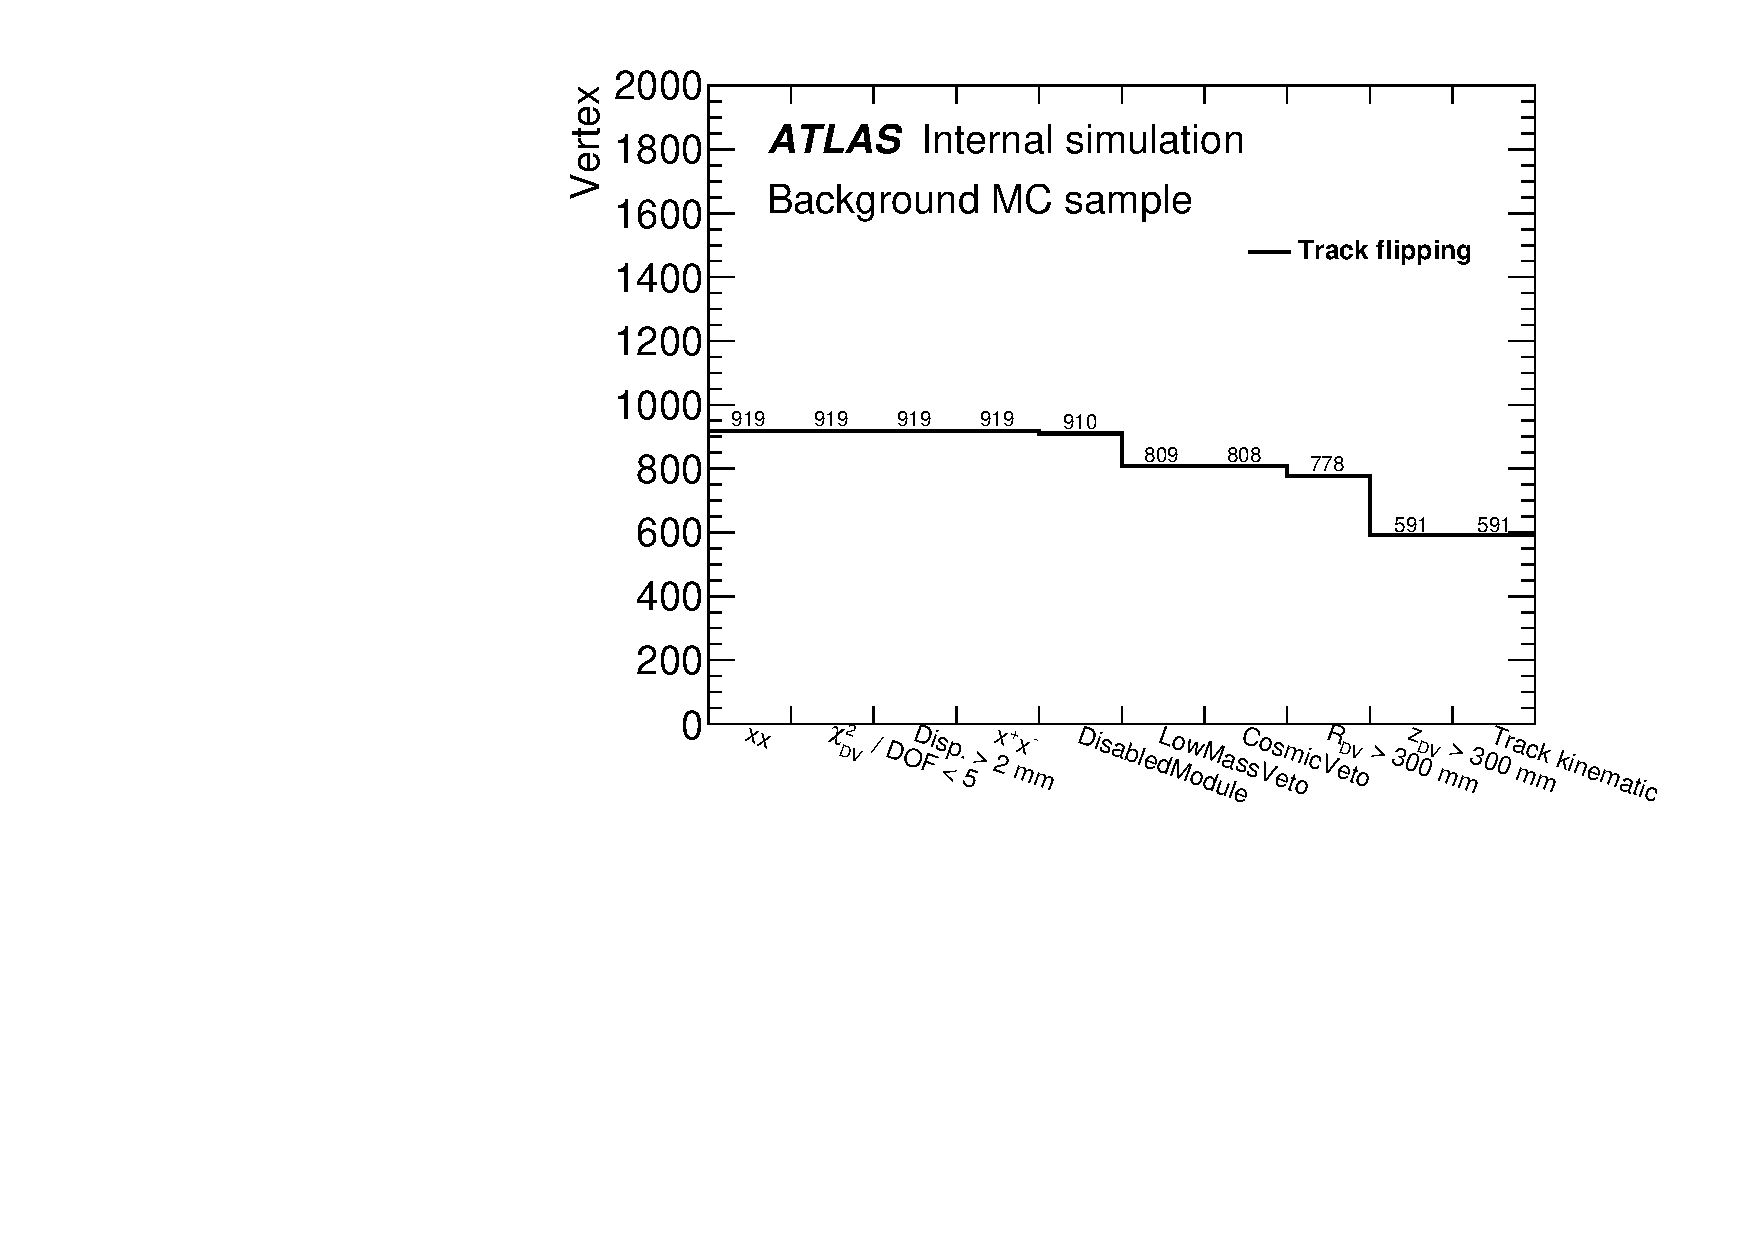
\includegraphics[width=0.60\textwidth]{figures/m_FBE_cutflow_MC.pdf}
	\centering
	\caption{Vertex cut flow applied on \xx vertices from the TF method.}
	\label{fig:m_FBE_cutflow_MC}
\end{figure}

The vertex yields from the TF and event mixing method, which represent the estimation for random-crossing background, are compared with the vertex yields from reconstruction in Table~\ref{table:random_vertex_count}. No random-crossing background of \mumu, \ee, or \emu type is expected from the MC samples using both methods. 
 
\begin{table}[!htb]
  \centering
  \begin{tabular}{ c  c c c }
    \hline
    \hline
	Vertex Type					& Track Flipping	        & Event Mixing	        & Background MC Samples \\
    \hline
	\mux						&	1						&	1.3 				&	0					\\
	\ex						    &	0						&	0.3 				&	1					\\
	\xx						    &	591 					&	714.0				&	497 				\\
    \hline
    \hline
  \end{tabular}
  \caption{Comparison of the number of \mux, \ex, and \xx vertices found in the TF and event mixing with those reconstructed in the background MC samples.}
  \label{table:random_vertex_count}
\end{table}

The \xx vertex yields from the TF and the event mixing methods agree within the statistical uncertainty. The kinematic distributions of the two tracks forming a vertex in TF and event mixing are compared with those of the background MC samples in Figure~\ref{fig:random-crossing_vertex_dist}. Both samples reproduce the distribution of vertex in the background MC samples.

\begin{figure}[!htb]
    \centering
    \subfloat[]{\label{subfig:random-crossing_MC_M}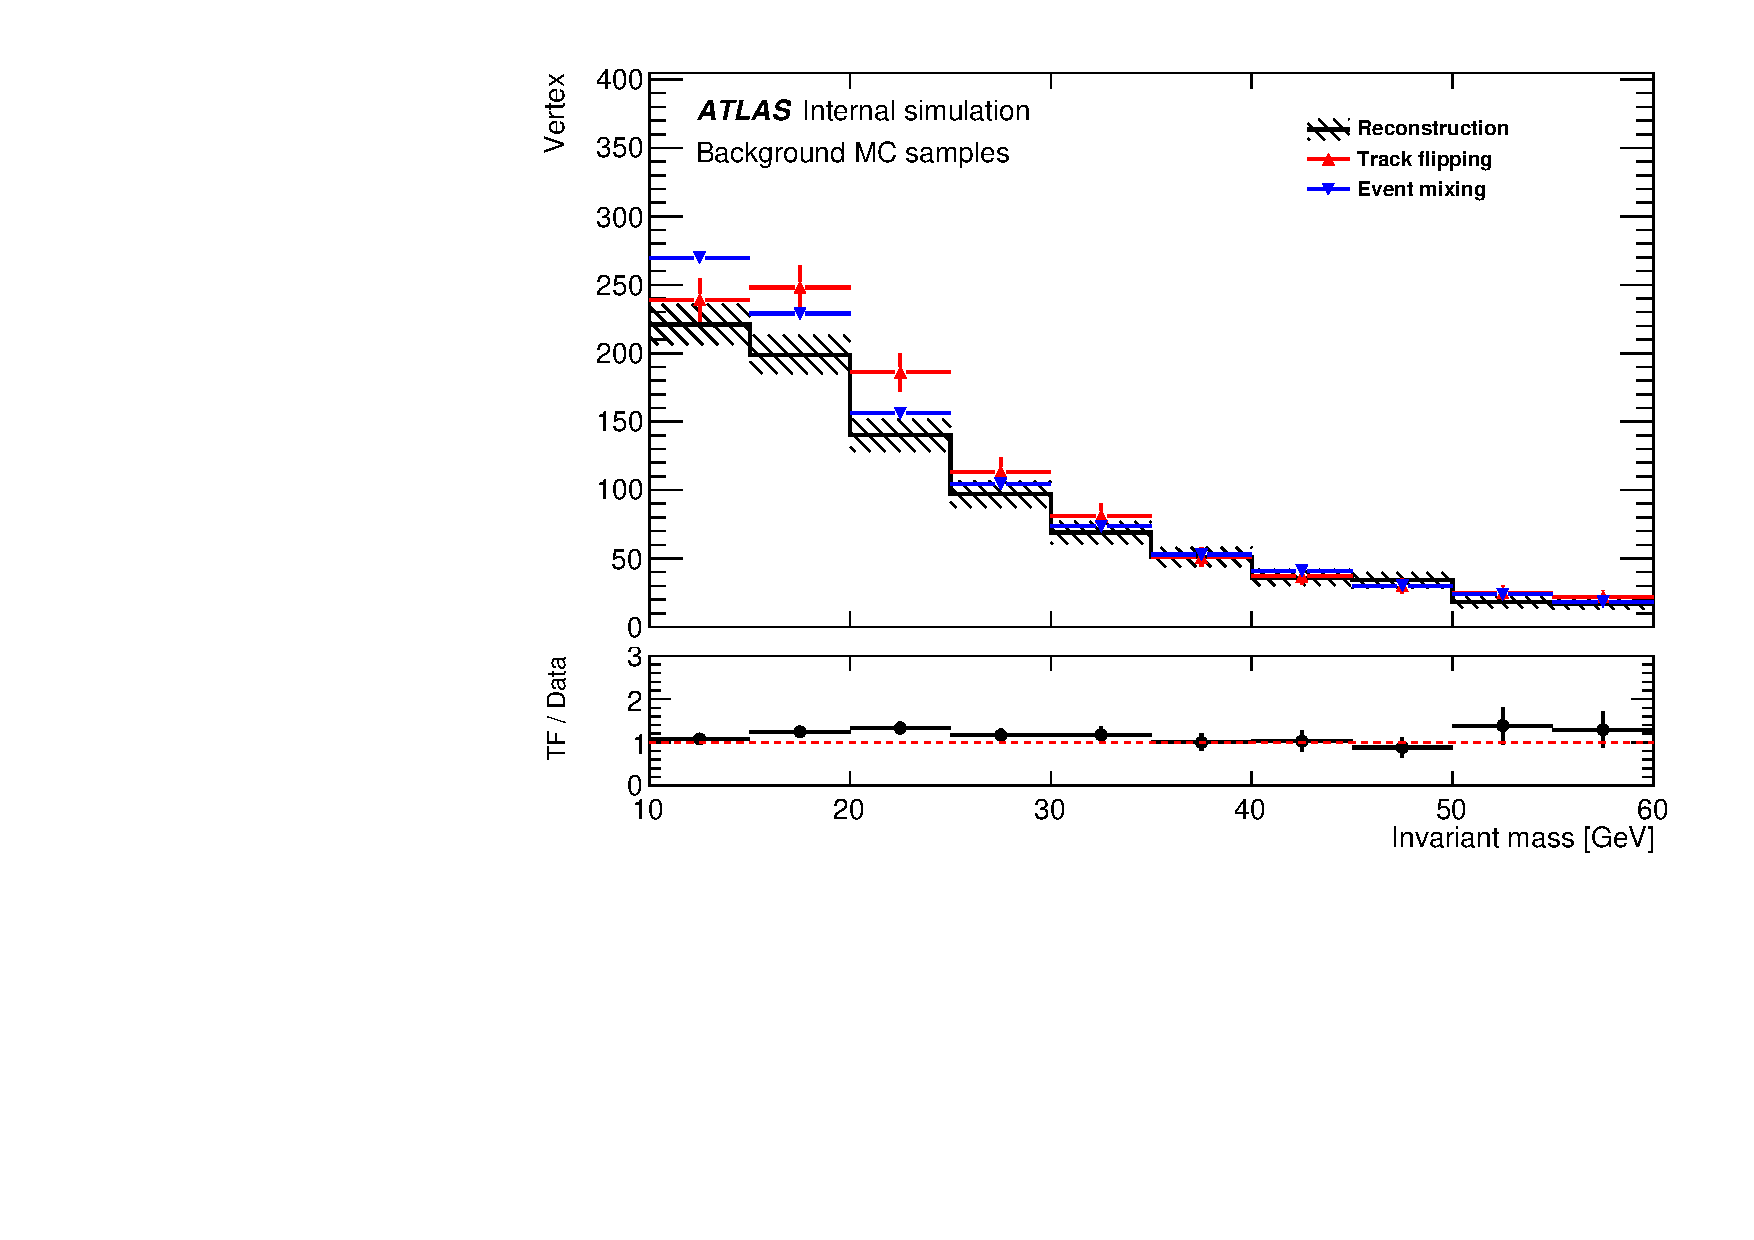
\includegraphics[width=0.45\textwidth]{figures/m_FBE_M.pdf}}
    \subfloat[]{\label{subfig:random-crossing_MC_chi2ndof}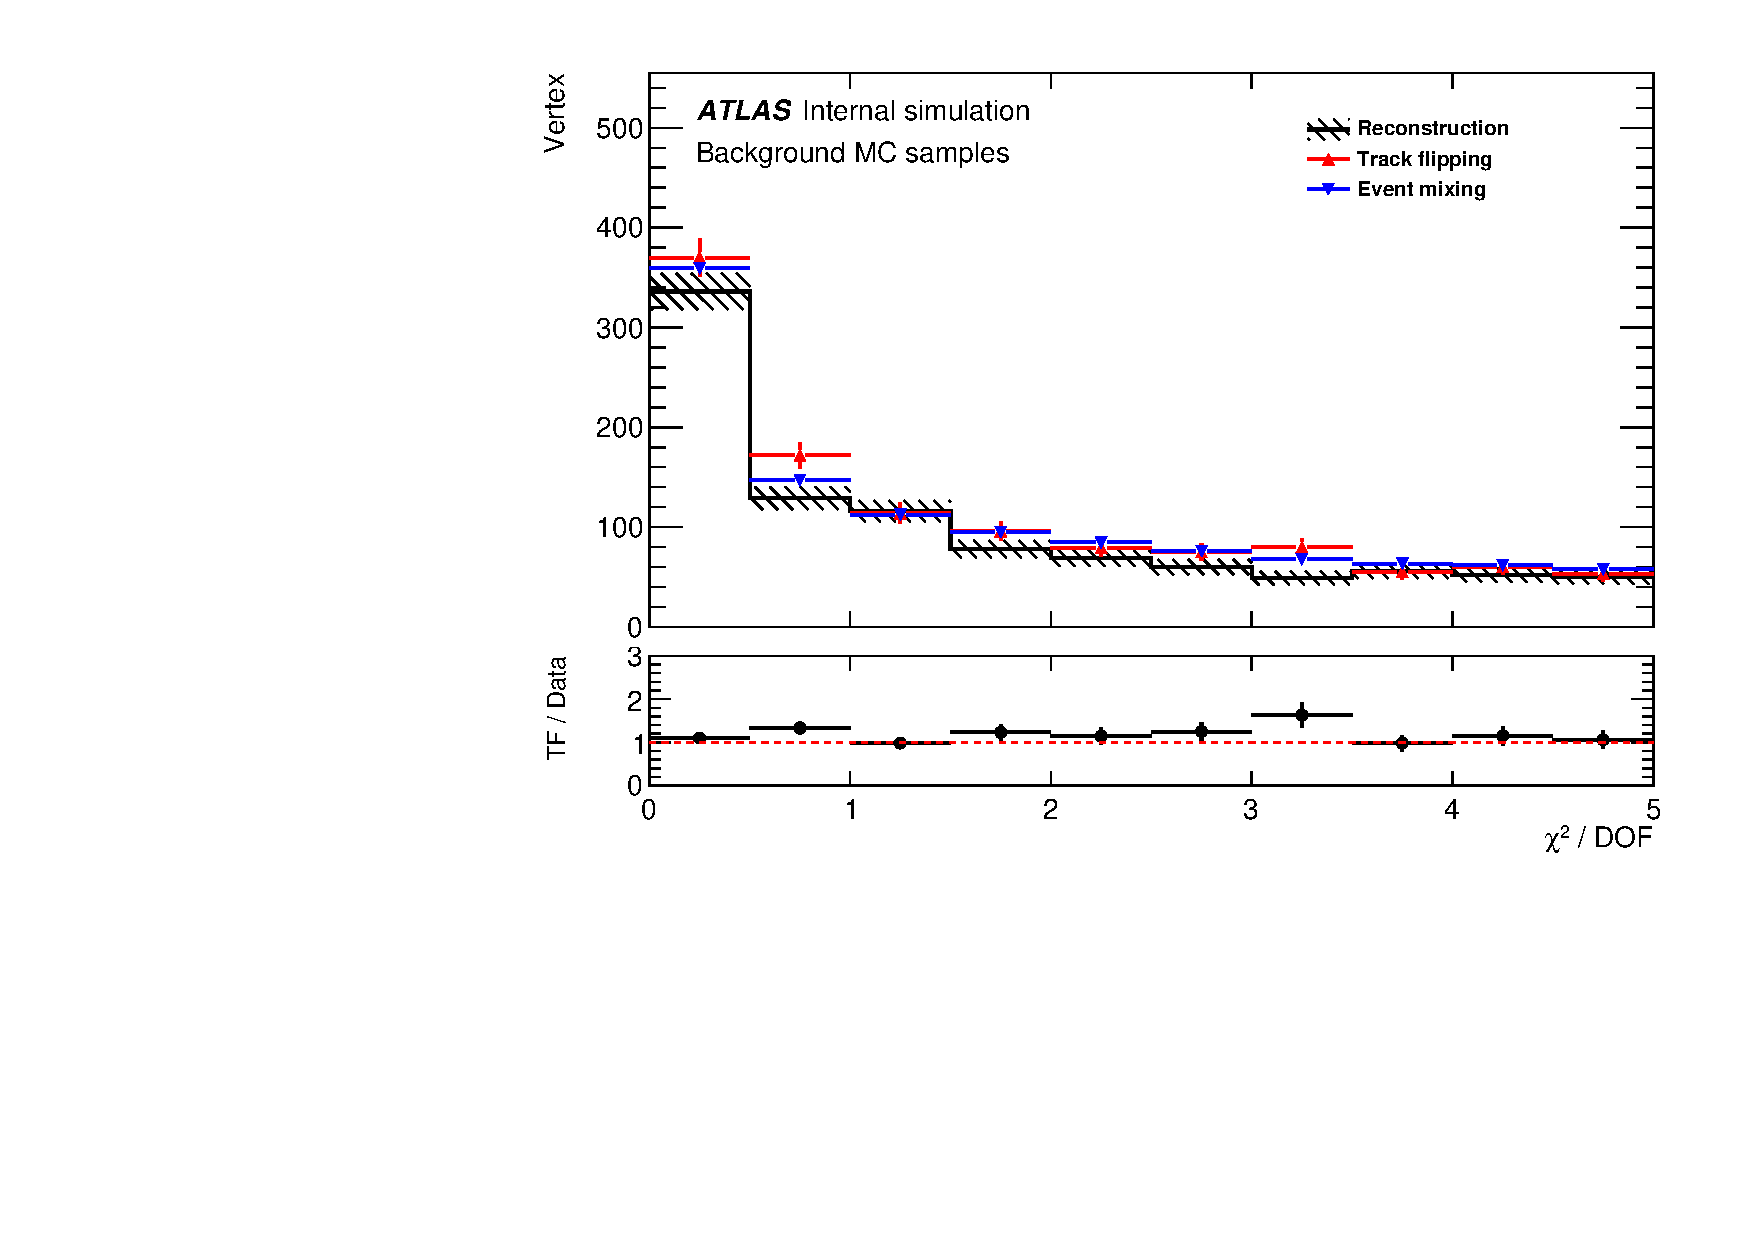
\includegraphics[width=0.45\textwidth]{figures/m_FBE_chi2_ndof.pdf}} \\
    \subfloat[]{\label{subfig:random-crossing_MC_r}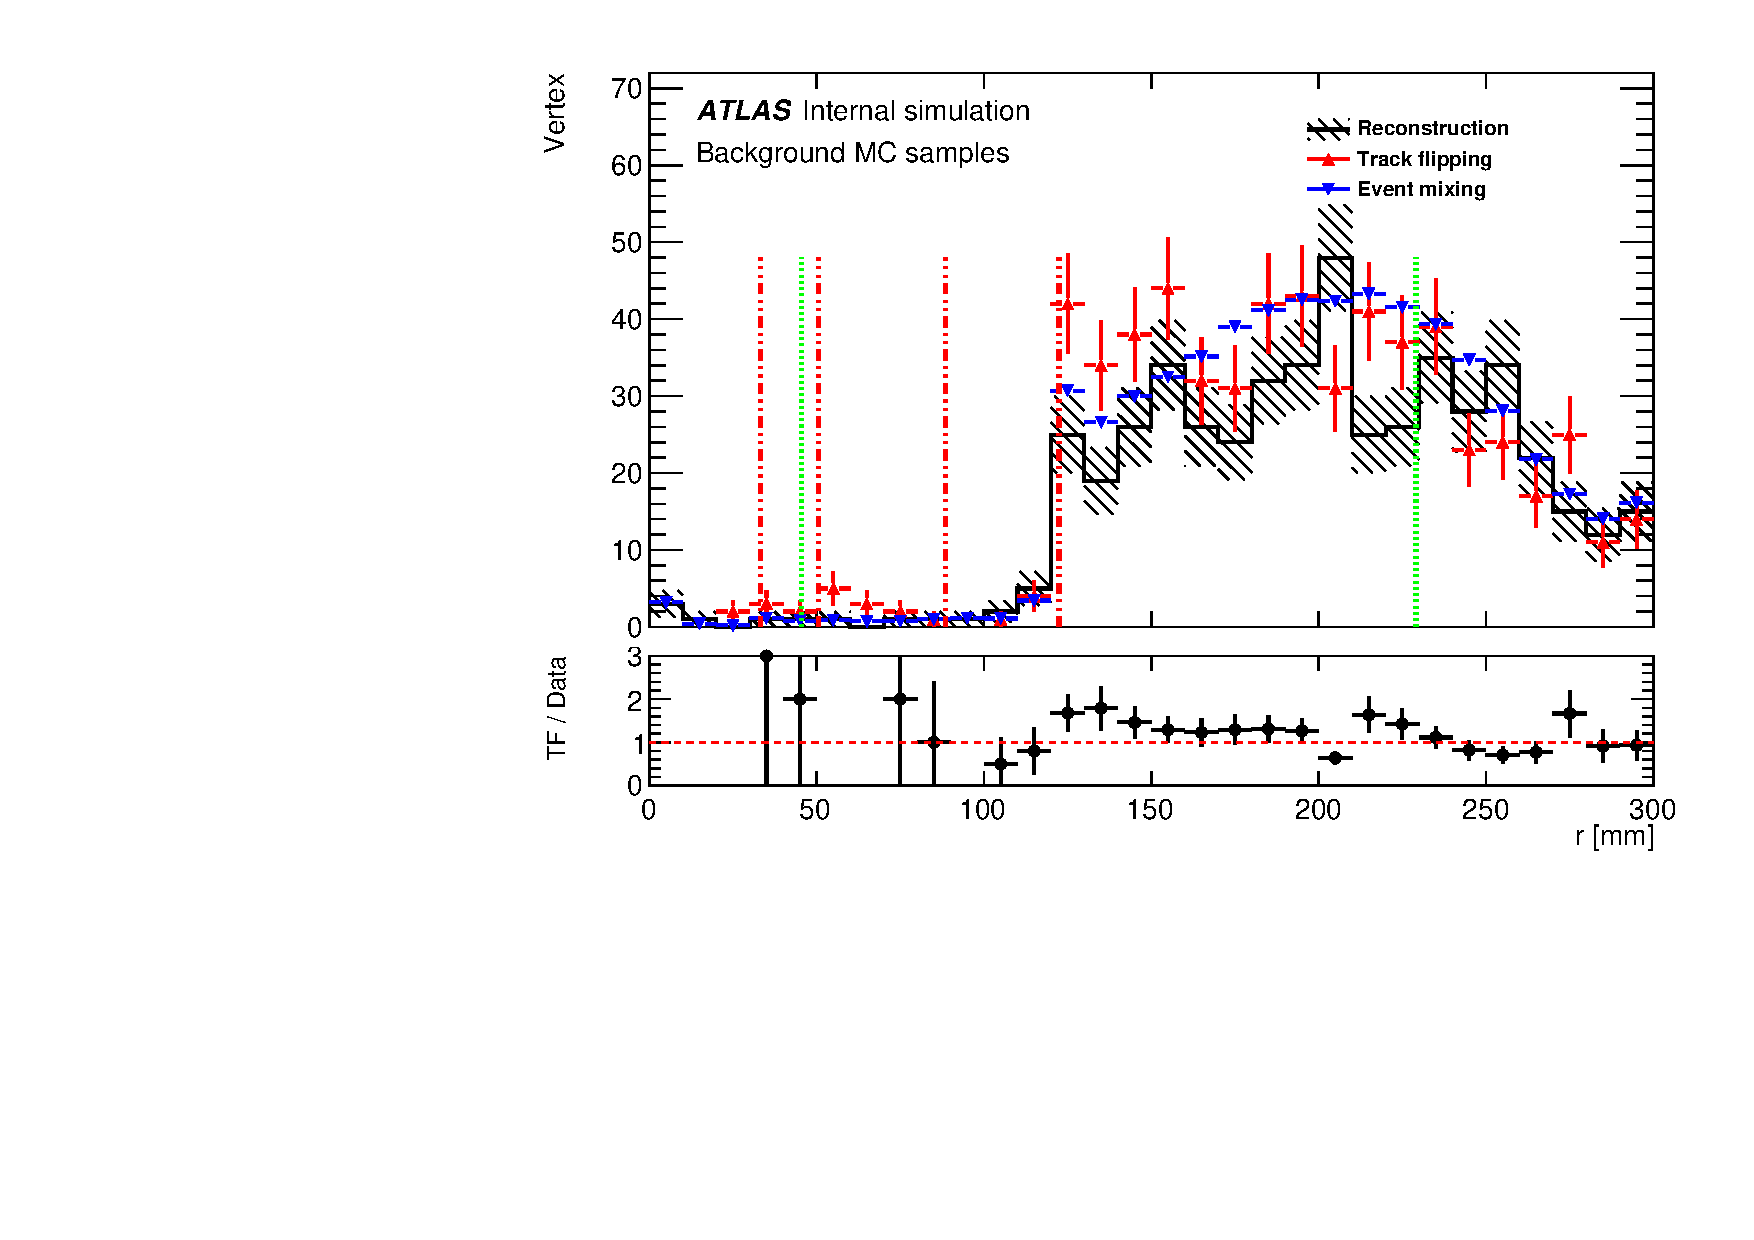
\includegraphics[width=0.45\textwidth]{figures/m_FBE_R.pdf}}
    \subfloat[]{\label{subfig:random-crossing_MC_z}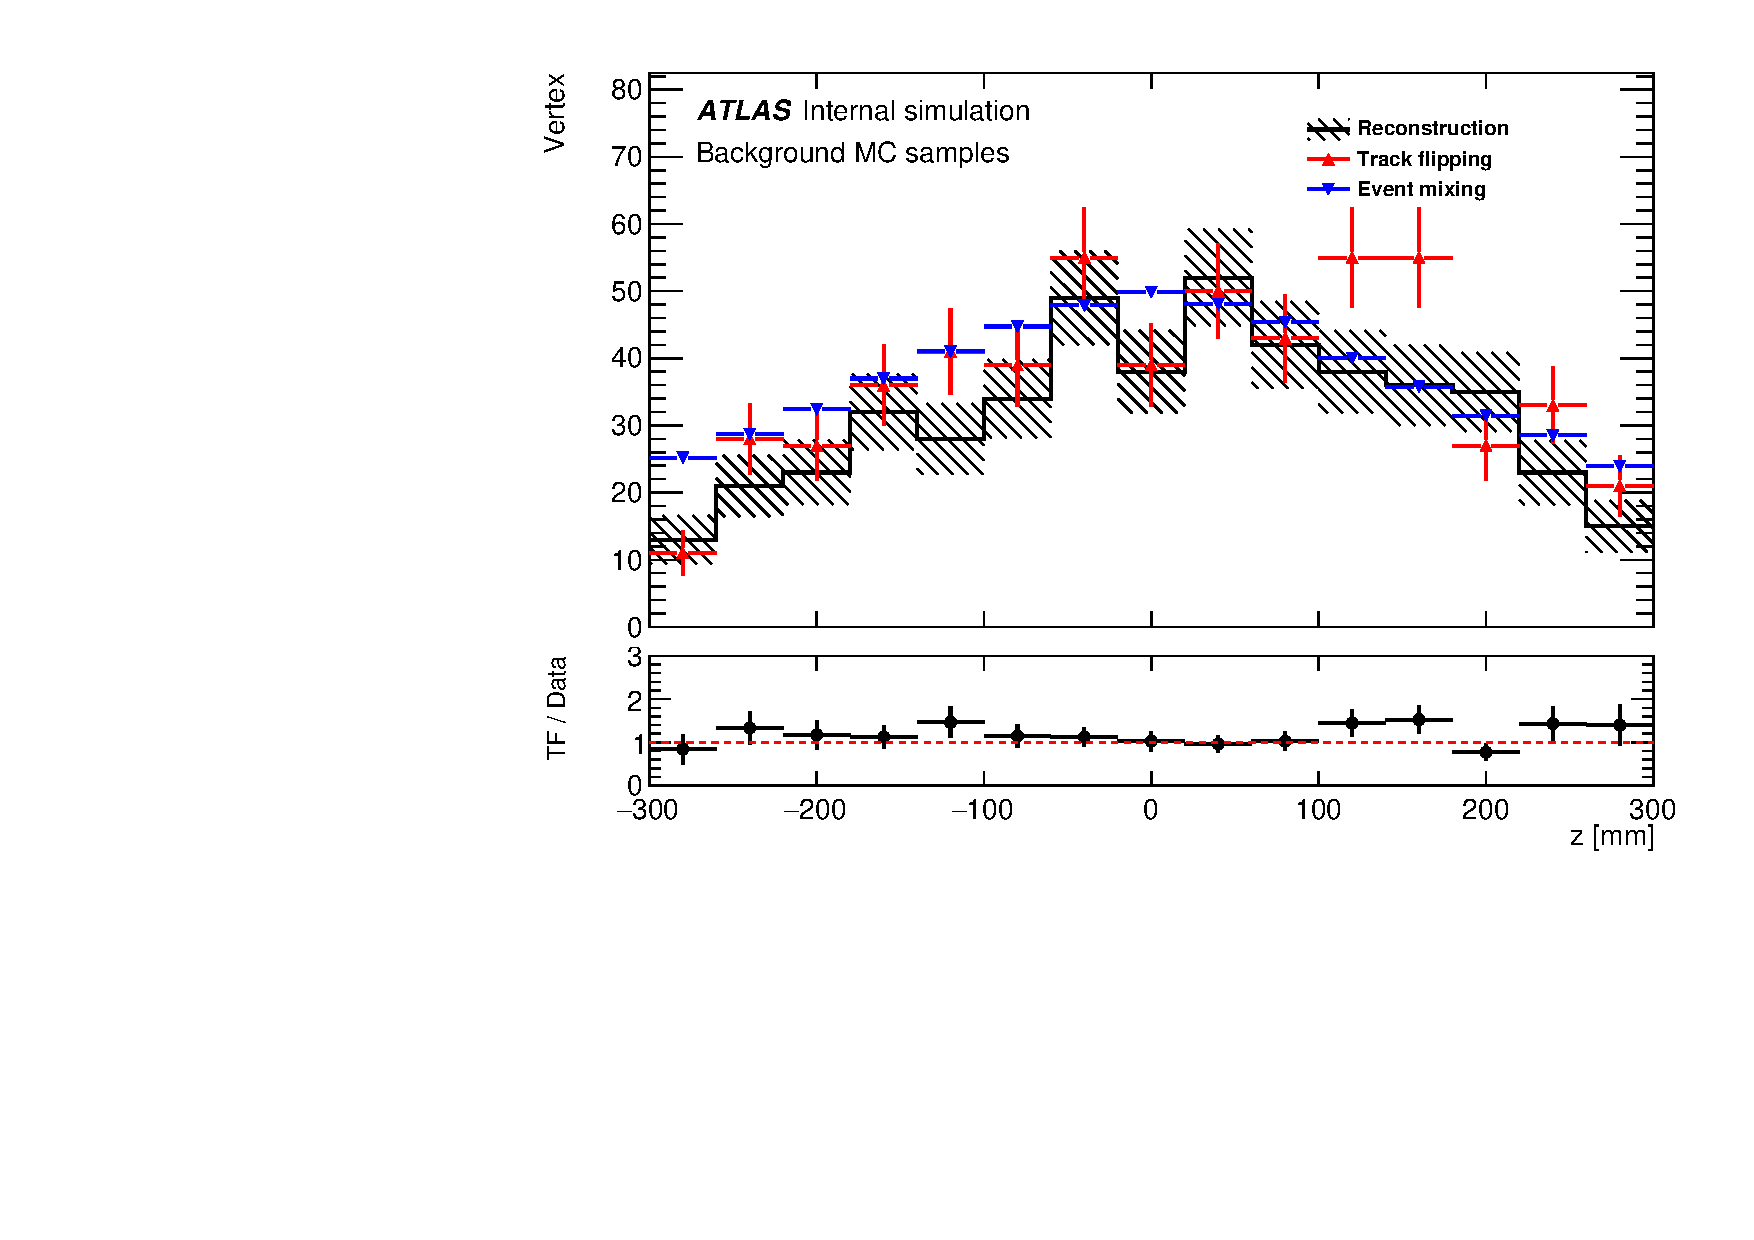
\includegraphics[width=0.45\textwidth]{figures/m_FBE_z.pdf}}
    %\subfloat[l]{\label{subfig:random-crossing_l}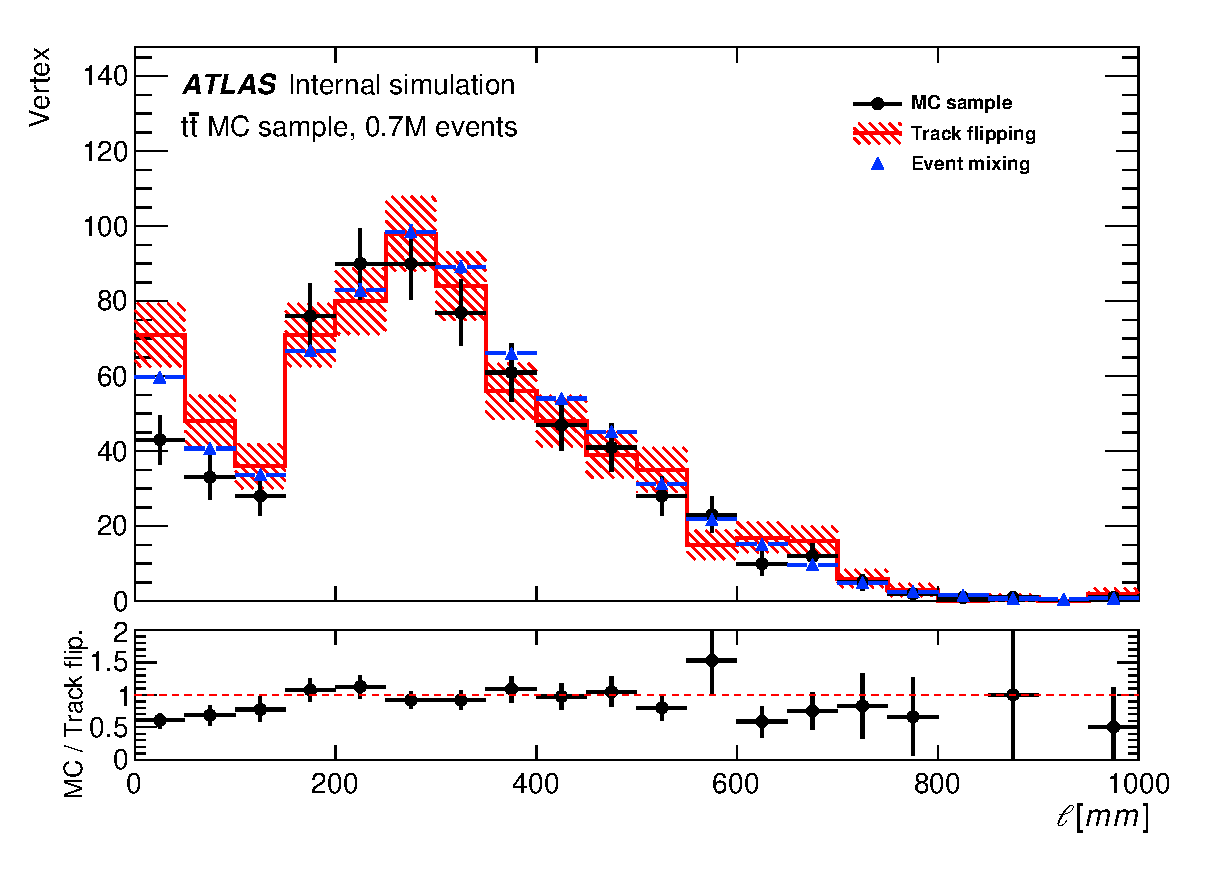
\includegraphics[width=0.45\textwidth]{figures/m_FBE_l.eps}}
    \caption{Comparison of of (a) vertex mass, (b) $\chi^{2} / \mathrm{DOF}$, (c) transverse, and (d) longitudinal position of \xx vertices reconstructed in TF and event mixing with those reconstructed in the background MC samples. In (c), the red dashed lines indicate the four Pixel layers. The green dotted lines indicate the Inner Support Tube (45.5 mm) and Pixel Support Tube (229 mm).}
    \label{fig:random-crossing_vertex_dist}
\end{figure}


\subsection{Estimating Random-crossing Background with Data Sample}
\label{sec:bkg:random_crossing_data}

Random-crossing background is estimated by performing the TF method on the data sample. Following the procedure described in Section~\ref{sec:bkg:random_crossing_tf}, track-flipped vertices are created, and the vertex yields in the control and validation regions can be used to estimate the random-crossing background in the signal region.

In the control region, the xx vertices found from the track flipping method are compared to the vertices reconstructed in the data sample in Figure~\ref{fig:random-crossing_vertex_dist_data}. The distributions shows that the TF method reproduces the data reasonably well including some of the structures of the ID, suggesting that the TF method provides a reasonable estimation of the random-crossing background.

\begin{figure}[!htb]
    \centering
    \subfloat[]{\label{subfig:random-crossing_M}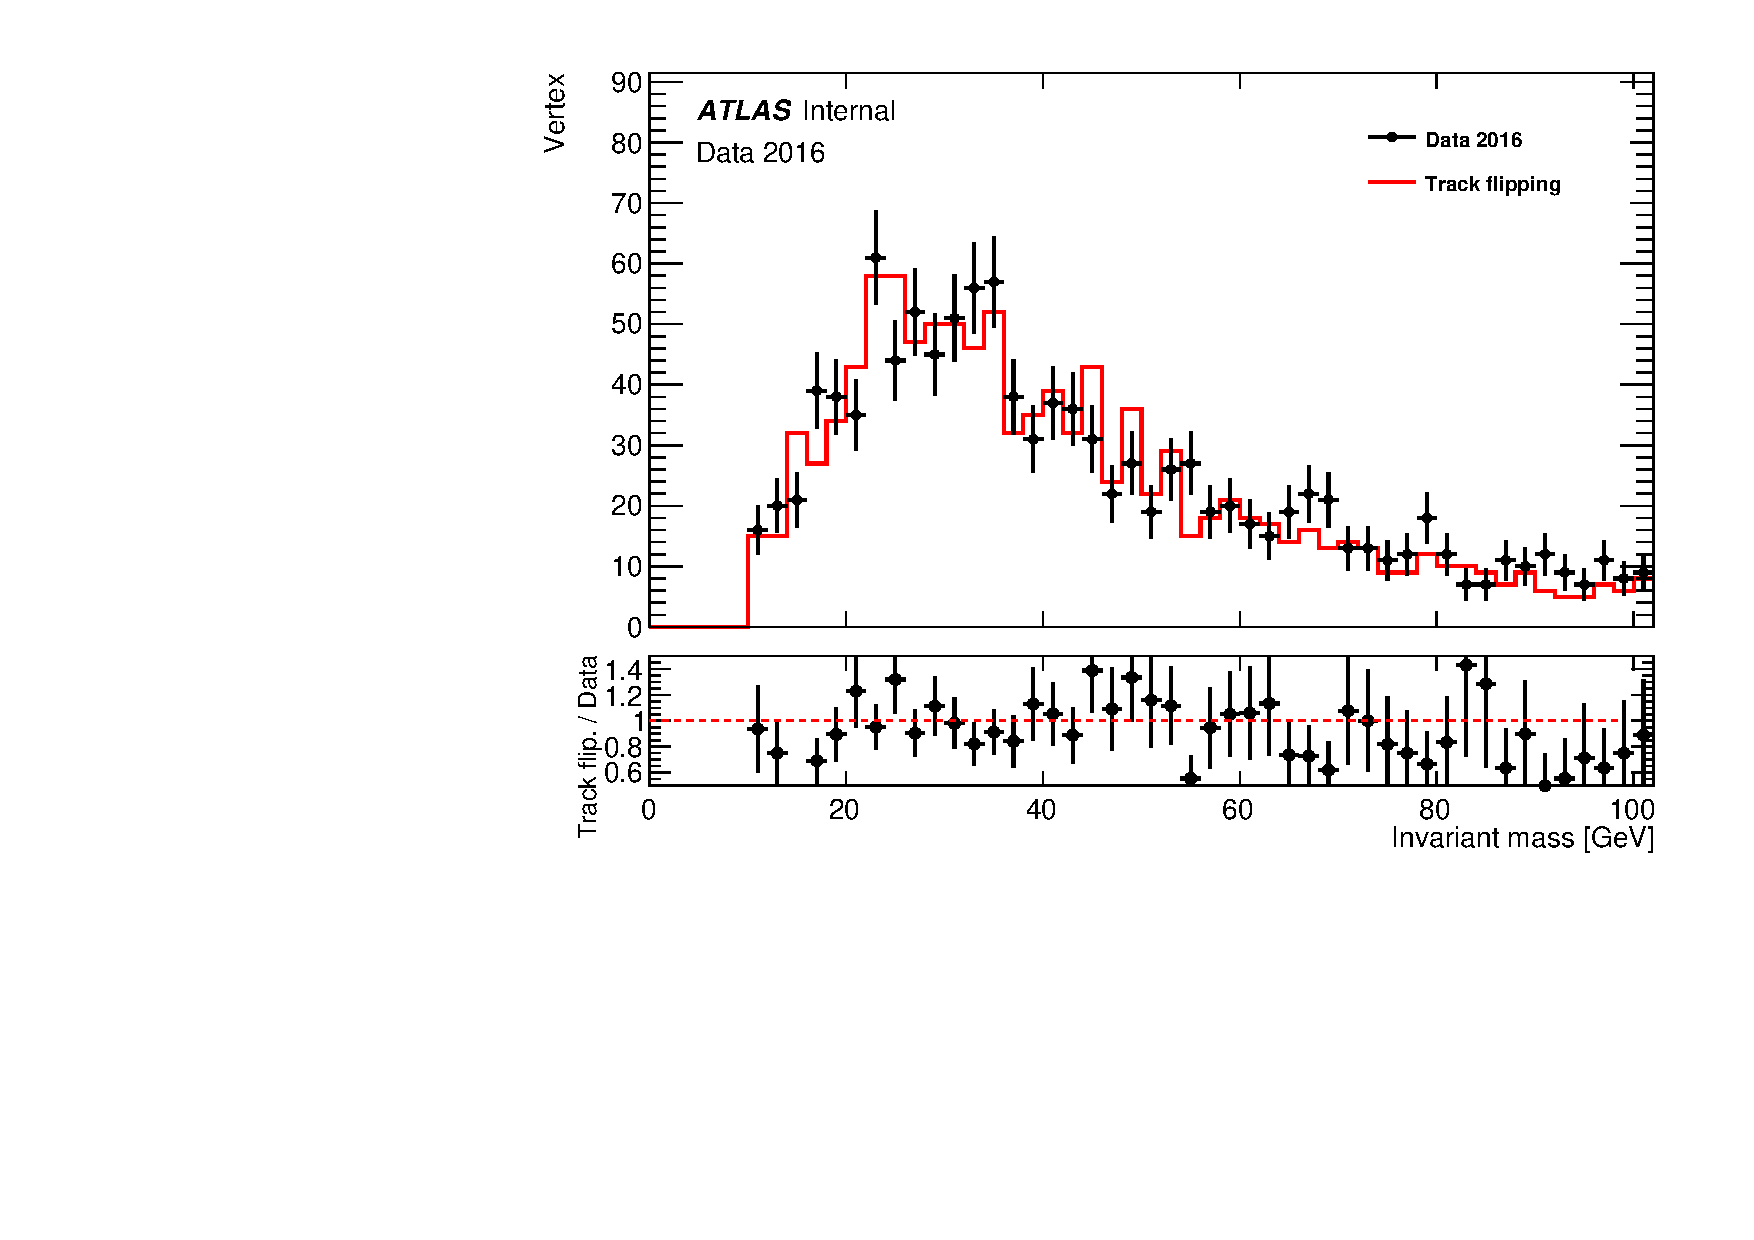
\includegraphics[width=0.45\textwidth]{figures/m_FBE_data_M.pdf}}
    \subfloat[]{\label{subfig:random-crossing_chi2ndof}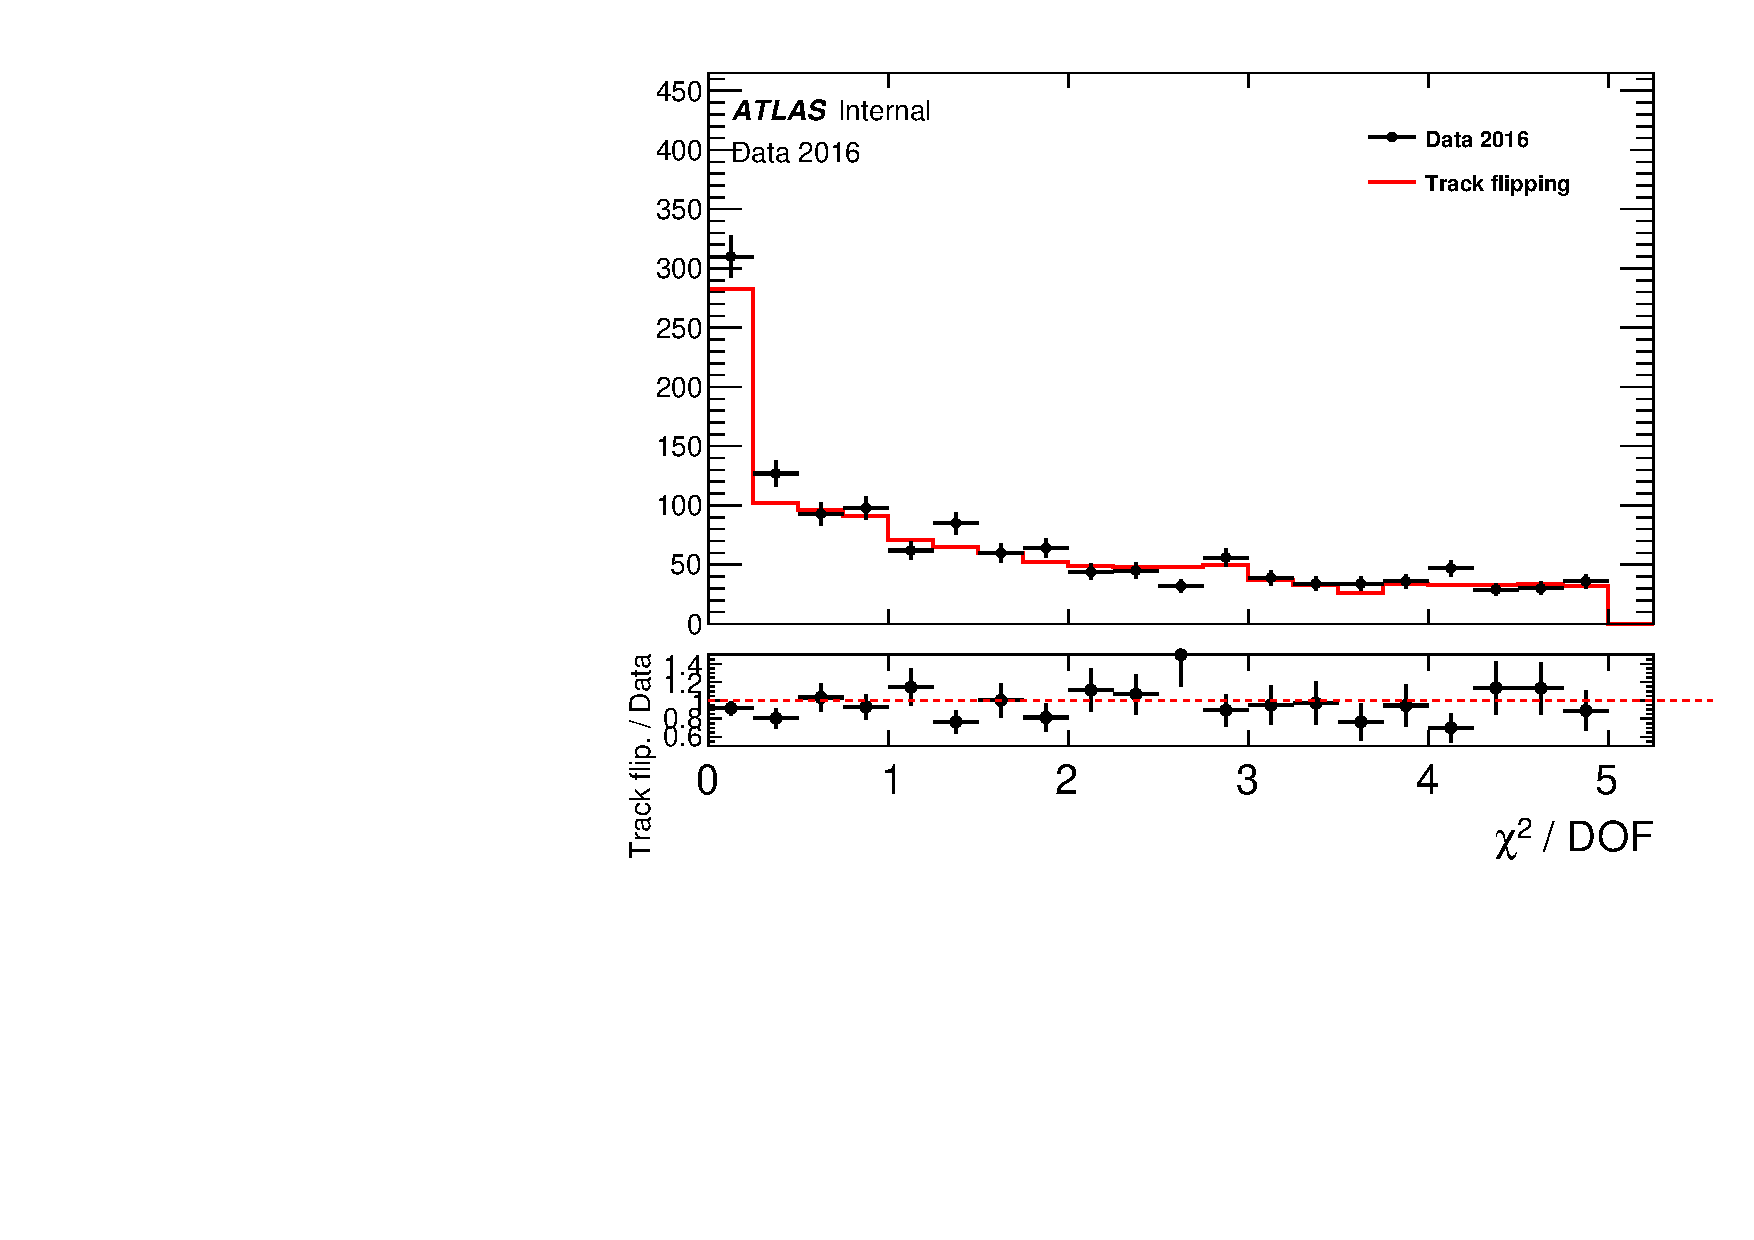
\includegraphics[width=0.45\textwidth]{figures/m_FBE_data_chi2_ndof.pdf}} \\
    \subfloat[]{\label{subfig:random-crossing_r}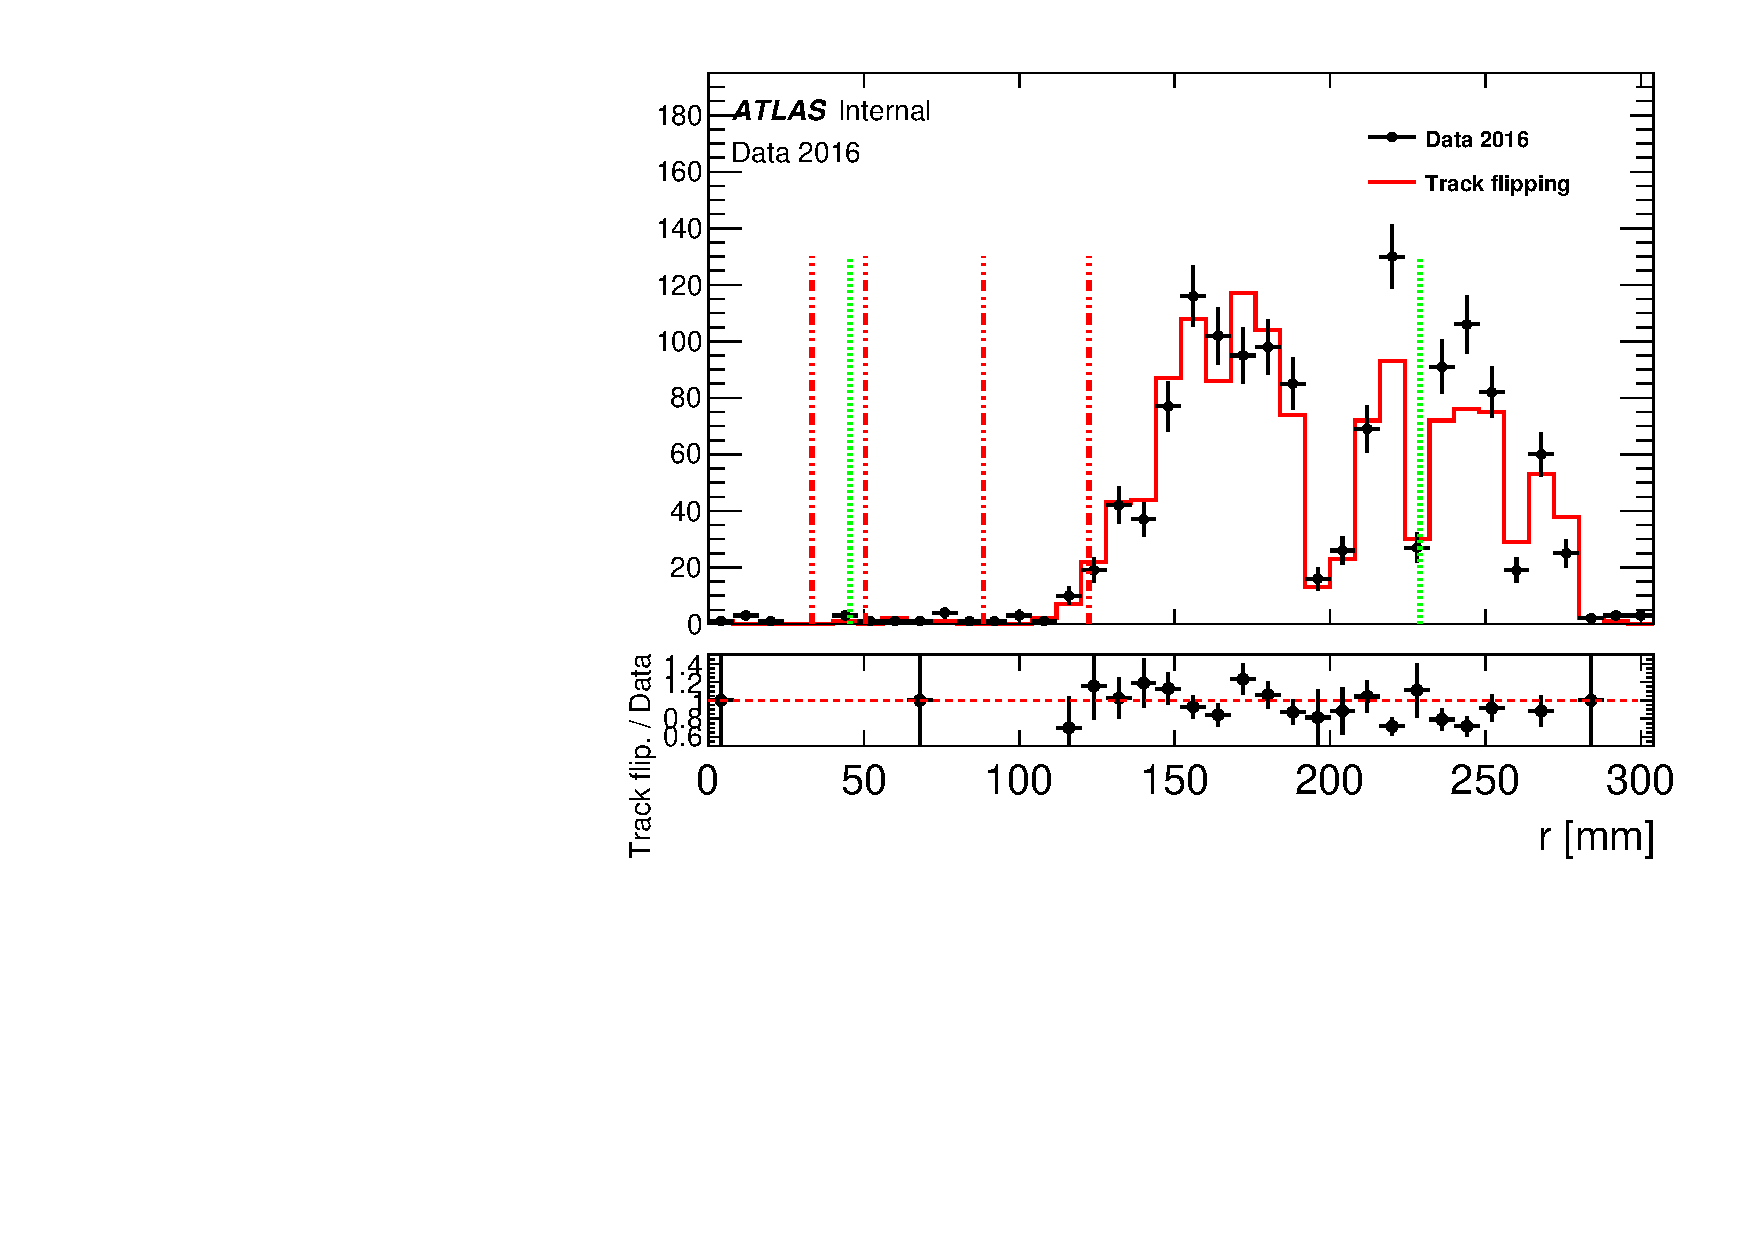
\includegraphics[width=0.45\textwidth]{figures/m_FBE_data_R.pdf}}
    \subfloat[]{\label{subfig:random-crossing_z}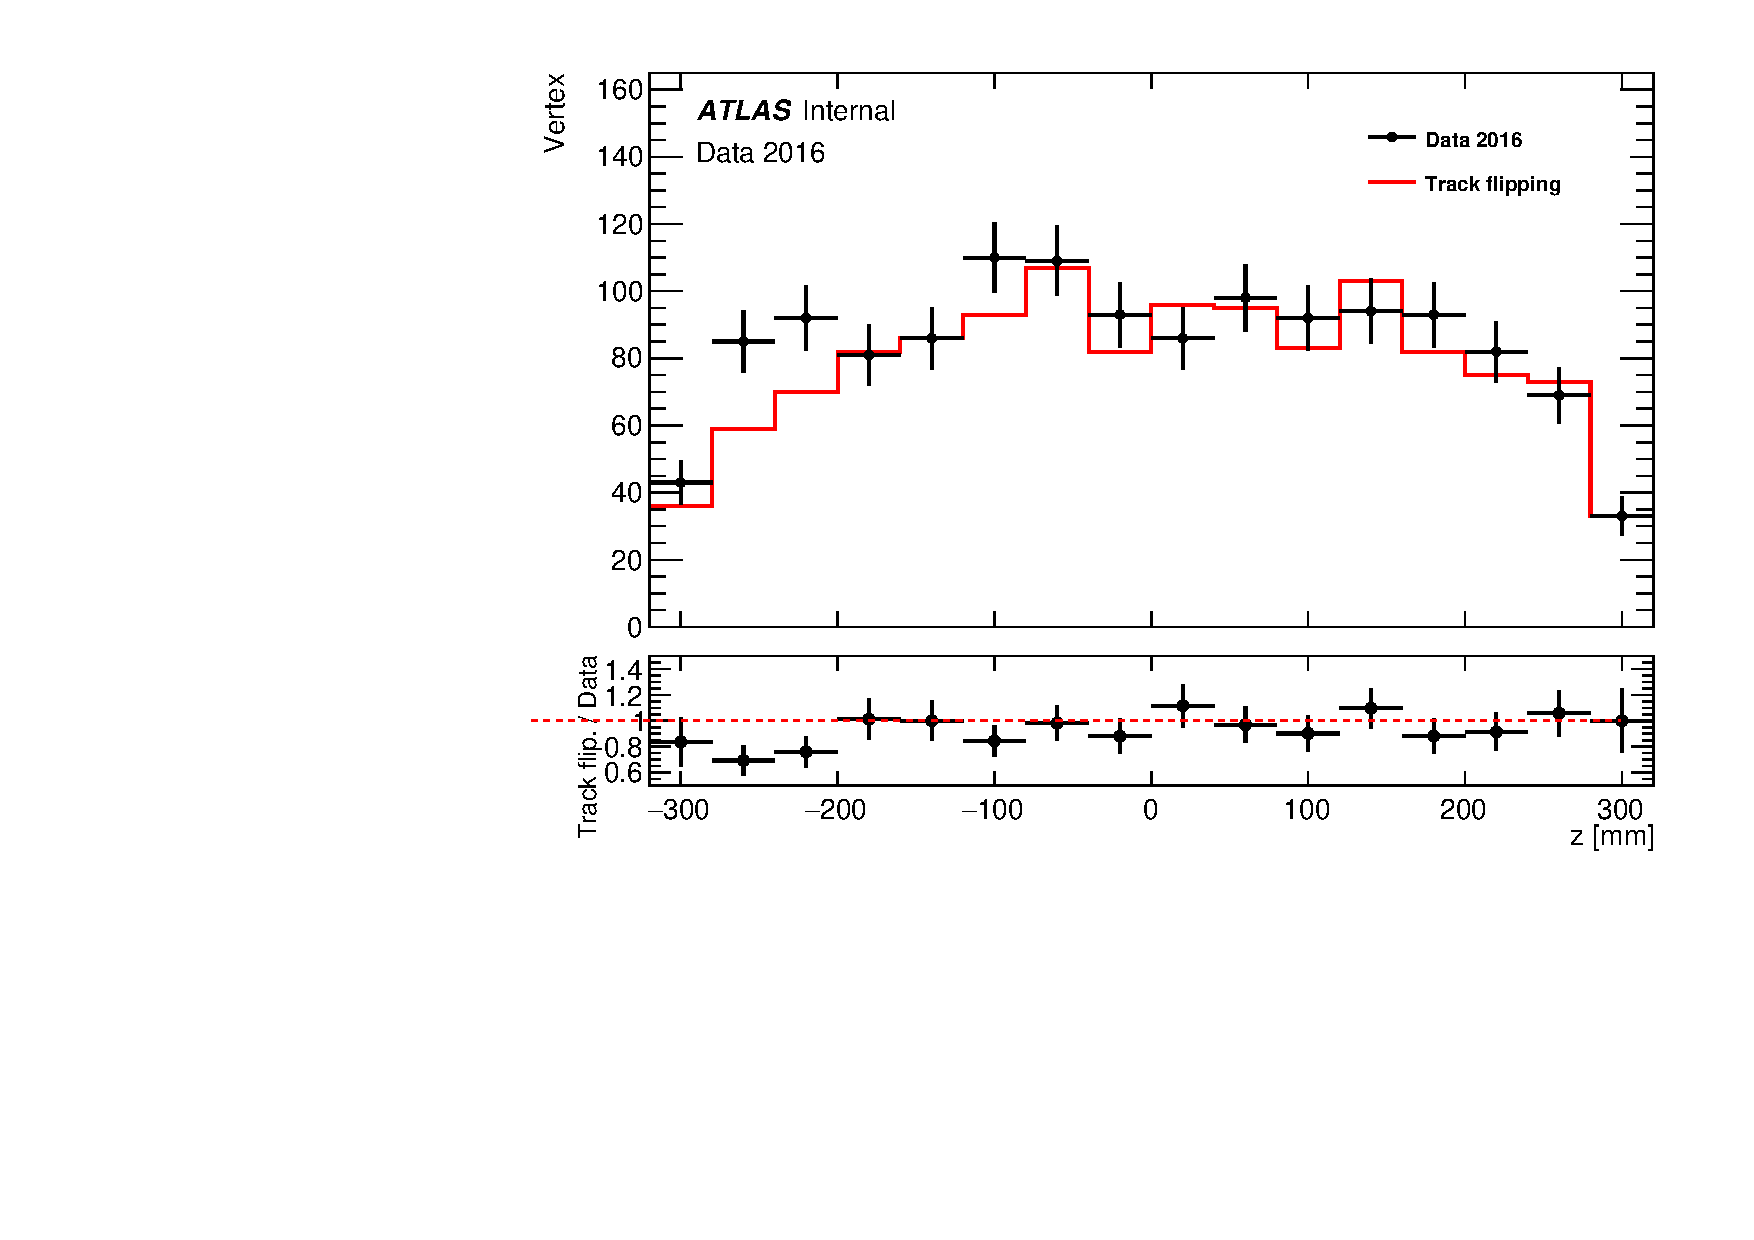
\includegraphics[width=0.45\textwidth]{figures/m_FBE_data_z.pdf}}
    %\subfloat[l]{\label{subfig:random-crossing_l}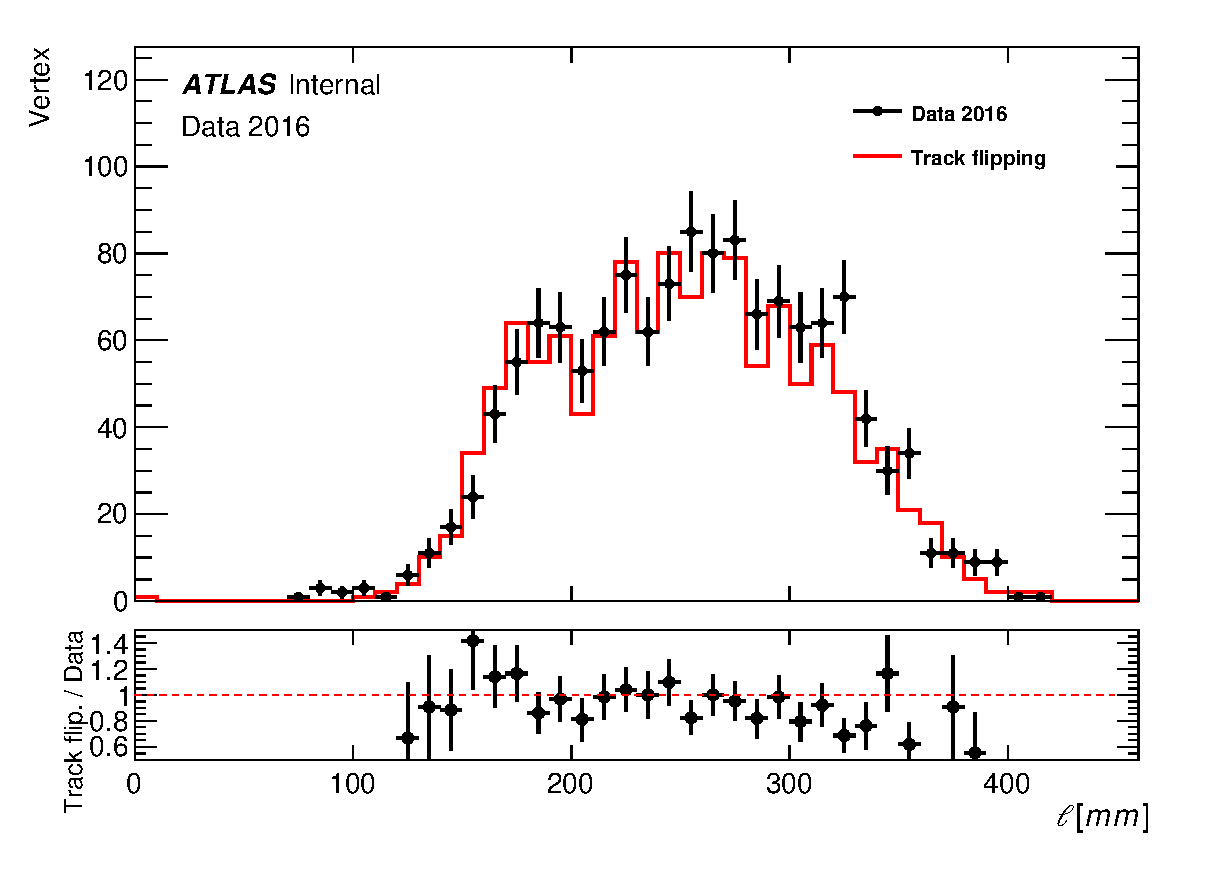
\includegraphics[width=0.45\textwidth]{figures/m_FBE_data_l.eps}}
    \caption{Comparison of (a) vertex mass, (b) $\chi^{2} / \mathrm{DOF}$, (c) transverse, and (d) longitudinal position of vertices found in data with vertices formed in track flipping in the control region. In (c), the red dashed lines indicate the four Pixel layers. The green dotted lines indicate the Inner Support Tube (45.5 mm) and Pixel Support Tube (229 mm).}
    \label{fig:random-crossing_vertex_dist_data}
\end{figure}

Because of the limited number in lepton pairs in the data sample, it is not practical to use the TF method to estimate the random-crossing background. Instead, the track-flipped vertex yields in the control region and validation region (region with zero or one lepton) are used to estimate random-crossing background in the signal region using the lepton probability, defined as follows:
\begin{itemize}
\item $P(e)$ is defined as the ratio of number of electrons to number of inner detector tracks in the entire sample,
\item $P(\mu)$ is defined as the ratio of number muons to number of inner detector tracks in the entire sample,
\end{itemize}
where track requirements described in Table~\ref{table:vertex_track_selection_simple} is imposed on both leptons and inner detector tracks. Lepton probability estimated from data is shown in Table~\ref{table:lepton_probability}.

\begin{table}[!htb]%
  \centering
    \begin{tabular}[t]{ccc}
        \hline\hline
                & Tracks             & P($\ell$)           \\
         \hline
         x      & $2.47\times10^{7}$ & -                   \\
         $\mu$  & $5.23\times10^{4}$ & $2.10\times10^{-3}$ \\
         $e$    & $3.63\times10^{4}$ & $1.46\times10^{-3}$ \\
         Sum    & $2.48\times10^{7}$ & - \\
        \hline\hline
    \end{tabular}
  \caption{Number of x, $\mu$, $e$ tracks and the calculated lepton probability from data.}%
  \label{table:lepton_probability}
\end{table}


Using the lepton probabilities, the track-flipping vertex yield in the control region (xx) is extrapolated into the validation region using Eq.~\ref{eq:TF_extrapolation_from_validation}, and the extrapolated $\mu$x and $e$x vertex yields are compared with the observed track-flipping vertex yield to determine scale factors as defined in Eq~\ref{eq:random_crossing_scale_factor}.

The track-flipping vertex yields in the control and validation regions are then extrapolated into the signal region using Eqs.~\ref{eq:TF_extrapolation_from_control}$-$\ref{eq:TF_extrapolation_from_validation} to estimate random-crossing background, and the scale factors (Eq.~\ref{eq:TF_scale_factors}) are applied to these extrapolation for more accurate estimation of the background.



%\textbf{Extrapolation from control region} The track-flipped vertex yields in the control region is extrapolated using Eq.~\ref{eq:TF_extrapolation_from_control} into the validation regions to estimate the vertex yields to test the validity of the TF method for estimating the random-crossing background. The estimated \mux and \ex vertex yields are compared with the observed track-flipped vertex yield in the region. The ratio of the observed track-flipped vertex to the extrapolated vertex in the validation region is used as scale factors for the estimation in the signal region,
%
%\begin{align}
%    S_{\mathrm{xx}\rightarrow \mu \mathrm{x}} &= \frac{N_{\mu \mathrm{x}}^{obs}}{N_{\mu \mathrm{x}}^{est}}, \nonumber \\
%    S_{\mathrm{xx}\rightarrow e\mathrm{x}}   &= \frac{N_{e\mathrm{x}}^{obs}}{ N_{e\mathrm{x}}^{est}}
%\label{eq:random_crossing_scale_factor}
%\end{align}
%where $N_{\mu \mathrm{x}}^{obs}$ and $N_{\mu \mathrm{x}}^{est}$ ($N_{e\mathrm{x}}^{obs}$ and $N_{e\mathrm{x}}^{est}$) represent the number of observed track-flipping vertex and the estimated vertex of each type.
%
%The track-flipped vertex yield is then extrapolated into the signal region using Eq.~\ref{eq:TF_extrapolation_from_control} to estimate random-crossing background after applying the scale factors defined by Eq.~\ref{eq:TF_scale_factors}.
%
%\textbf{Extrapolation from validation region} Similarly, the track-flipped vertex yields in the validation region is extrapolated into the signal region to estimate vertex yields using Eq.~\ref{eq:TF_extrapolation_from_validation} after applying the scale factor defined by Eq.~\ref{eq:TF_scale_factors}.

The raw vertex yields in the TF method and data, and the scale factors calculated from the vertex yields are presented in Appendixs~\ref{sec:tf_raw_yields}. The final estimate of random-crossing background from the TF method are shown in Table~\ref{table:track_flipping}. The estimate of the background after applying the scale factors in the signal region is $3.95\times10^{-3}$, which is compatible with the corresponding result of $2.40\times 10^{-3}$ from the event mixing method~\cite{DuarteCampderros:2275055}.


\begin{table}[!htb]%
  \centering
  \resizebox{\textwidth}{!}{
    \begin{tabular}[t]{cccc}
        \hline\hline
                                  & Raw estimate from xx & Raw estimate from $\mu$x, $e$x & Corrected estimate  \\
         \hline
         $N_{\mu\mu}$             & $2.69\times10^{-3}$  & $2.19\times10^{-3}$            & $1.79\times10^{-3}$ \\
         $N_{ee}$                 & $5.56\times10^{-3}$  & $1.05\times10^{-3}$            & $1.99\times10^{-4}$ \\
         $N_{e\mu}$               & $7.73\times10^{-3}$  & $3.89\times10^{-3}$            & $1.96\times10^{-3}$ \\
         \hline
         Sum of signal regions    & $1.60\times10^{-2}$  & $7.13\times10^{-3}$            & $3.95\times10^{-3}$ \\
        \hline\hline
    \end{tabular}
  }
  \caption{The estimate of random-crossing background in the signal region. Scale factors (Table~\ref{table:tf_raw_yields}) are applied to obtain the corrected estimate of the background.}%
  \label{table:track_flipping}
\end{table}




